\documentclass[12pt]{article}
\usepackage[margin=1.0in]{geometry} %page layout
\usepackage[usenames,dvipsnames]{color} %color
\definecolor{light-gray}{gray}{0.95}
\definecolor{darkgreen}{rgb}{0,0.4,0}
\usepackage{graphicx, subfigure} %figures
\usepackage{url, hyperref} %cross-referencing
\usepackage{amsmath, amssymb} %math
\usepackage{listings} %source code
\lstset{breaklines=true,
breakindent=0pt,
prebreak=\mbox{\tiny$\searrow$},
postbreak=\mbox{{\color{blue}\tiny$\rightarrow$}},
numbers=left,
commentstyle=\color{darkgreen},
numberblanklines=false,
frame=single,
captionpos=b,
backgroundcolor=\color{light-gray}}
\usepackage[3D]{movie15} %for movies (needs hyperref)
	\newenvironment{changemargin}[2]
	{
	  	\begin{list}{}
		{
			\setlength{\topsep}{0pt}%
			\setlength{\leftmargin}{#1}%
			\setlength{\rightmargin}{#2}%
			\setlength{\listparindent}{\parindent}%
			\setlength{\itemindent}{\parindent}%
			\setlength{\parsep}{\parskip}%
		}
	  	\item[]
		}
		{\end{list}
	}
\author{Salman Aslam\\Georgia Tech}
\title{Tracking Results}
\date{}
\begin{document}
\maketitle
\rule[0pt]{\textwidth}{1pt}
\tableofcontents
\rule[0pt]{\textwidth}{1pt}
%=========================
\section{Introduction}
%=========================
In this report, our goal is to present tracking error results for our 6 different trackers, PCA-based, TSVQ-based and 4 RVQ-based trackers, maxP, RofE, nulE, and monR.


								\begin{figure}[t]
								\centering
								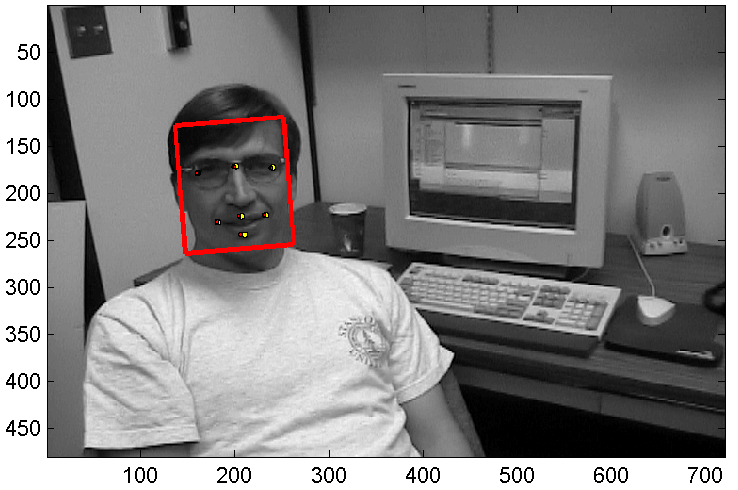
\includegraphics[width=0.7\textwidth]{temp/results_pca__trk_dudek_0007.png}
								\caption{Computing tracking error.  The larger yellow circles indicate ground truth feature points.  The smaller red circles indicate estimated feature points.  Tracking error is computed using the rms error between the ground truth feature points and the estimated feature points.  In this particular frame, the tracking error is 2.57.}
								\label{fig:results_pca__trk_dudek_0007}
								\end{figure}
%=========================
\section{Experiments}
%=========================
We have previously described our 5-component tracker comprising appearance, observation, representation, motion and inference models.  All 6 trackers share exactly the same representation, motion and inference models.  However, each has its own appearance and observation models.

All trackers were run on 6 publicly available datasets, Dudek, davidin300, sylv, fish, car4 and car11.  See Figure~\ref{fig:trk_sequences} in Appendix~\ref{App:dataset_snapshots} for snapshots of images in each dataset at 100 image intervals.  These datasets can be downloaded from~\cite{2008_JNL_subspaceTRK_Ross}.  Tracking error was measured on each of these datasets using the error between ground truth feature points and estimated feature points as shown in Figure~\ref{fig:results_pca__trk_dudek_0007} for the Dudek sequence.

								\begin{figure}[t]
								\centering
								\begin{tabular}{|l|c|c|c|c|c|c|}
\hline
&\textbf{PCA}&\textbf{TSVQ}&\textbf{maxP}&\textbf{RofE}&\textbf{nulE}&\textbf{monR}\\\hline
\textbf{Dudek}&7.44&8.62&7.78&7.11&7.97&8.73\\\hline
\textbf{davidin300}&4.60&5.93&4.47&5.74&4.63&4.15\\\hline
\textbf{sylv}&4.34&4.61&4.00&4.12&4.74&4.31\\\hline
\textbf{fish}&2.17&4.59&2.78&2.73&2.48&2.89\\\hline
\textbf{car4}&4.60&5.11&4.67&4.93&5.28&4.71\\\hline
\textbf{car11}&2.13&2.21&2.17&2.33&2.52&2.47\\\hline
\textbf{ \% best}&50.00&0.00&16.67&16.67&0.00&16.67\\\hline
\end{tabular}

								\subfigure[Best tracking error for each algorithm.]{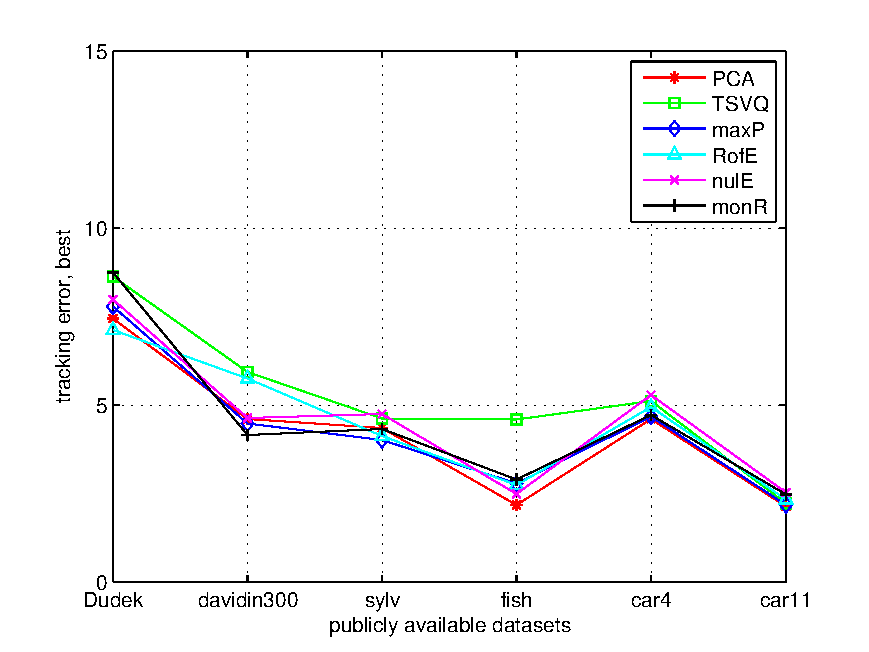
\includegraphics[width=0.47\textwidth]{temp/results_final_1a_best.pdf}\label{fig:results_final_1a_best}}
								\subfigure[]{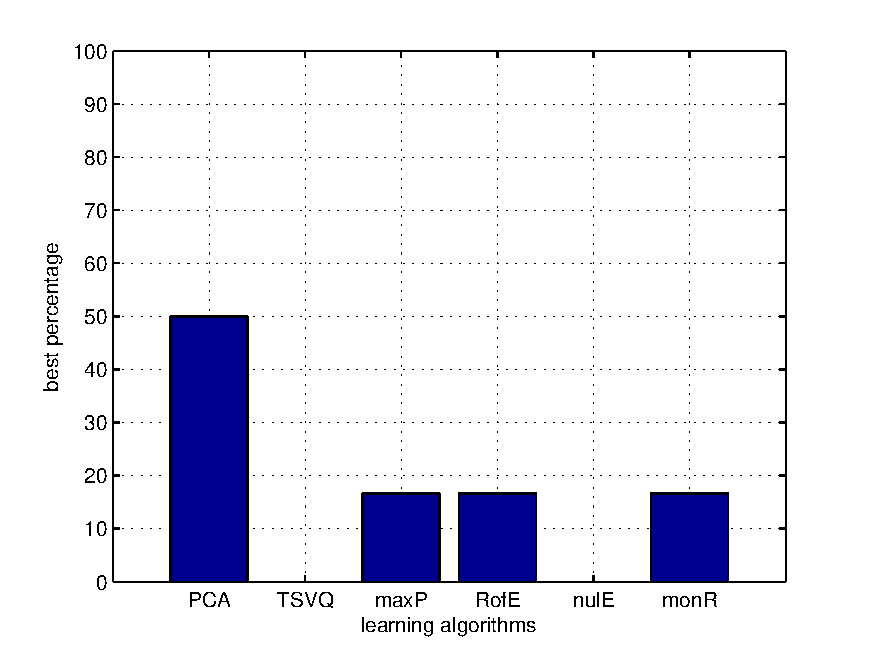
\includegraphics[width=0.47\textwidth]{temp/results_final_1b_best_percent.pdf}\label{fig:results_final_1b_best_percent}}
								\caption{Tracking results (1 of 5), comparison of best tracking performance.  PCA give best performance for half the datasets, i.e. 3 datasets, while RVQ gives best performance for the other half.}
								\label{fig:results_final_1_best}
								\end{figure}

Experimental results are given in Figures~\ref{fig:results_final_pca_}, \ref{fig:results_final_tsvq}, \ref{fig:results_final_maxP}, \ref{fig:results_final_RofE} \ref{fig:results_final_nulE} and \ref{fig:results_final_monR} in Appendix~\ref{App:tracking_error_plots} for PCA, TSVQ, maxP, RofE, nulE and monR respectively.  Results derived from these figures are explained in the results section.  Each of the 6 figures mentioned comprises a table and 4 plots.  Each entry in a table represents tracking error temporally averaged over the frames of a dataset (most of the datasets have more than 500 images).  The entries in a table are visualized in the accompanying 4 plots.  The plots show tracking error for different parameter values and their averages, and tracking error for different datasets and their averages.  

For the datasets, we make the following observations:

\begin{enumerate}
\item The Dudek and davidin300 sequences have lighting changes, pose changes, structured noise (putting on and taking off glasses) and expression changes.  In addition, the Dudek sequence has temporary occlusions and sudden motion.  These two sequences can be considered to be the most challenging datasets since they both have several different forms of noise.  A significant form of noise is blur due to sudden motion.  
\item The fish sequence has sudden lighting changes and sudden motion.
\item Sylv, car4 and car11 sequences have relatively less variation in lighting and pose.
\end{enumerate}

								\begin{figure}[t]
								\centering
								\begin{tabular}{|l|c|c|c|c|c|c|}
\hline
&\textbf{PCA}&\textbf{TSVQ}&\textbf{maxP}&\textbf{RofE}&\textbf{nulE}&\textbf{monR}\\\hline
\textbf{Dudek}&7.93&10.07&7.93&7.91&8.60&9.90\\\hline
\textbf{davidin300}&6.63&8.37&7.07&6.99&5.72&4.99\\\hline
\textbf{sylv}&5.18&4.70&4.47&4.83&5.10&4.66\\\hline
\textbf{fish}&6.63&6.71&8.81&5.97&5.74&6.15\\\hline
\textbf{car4}&4.97&5.90&5.38&5.19&5.77&4.99\\\hline
\textbf{car11}&2.24&3.48&2.70&2.49&2.69&2.58\\\hline
\textbf{ \% best}&33.33&0.00&16.67&16.67&16.67&16.67\\\hline
\end{tabular}

								\subfigure[]{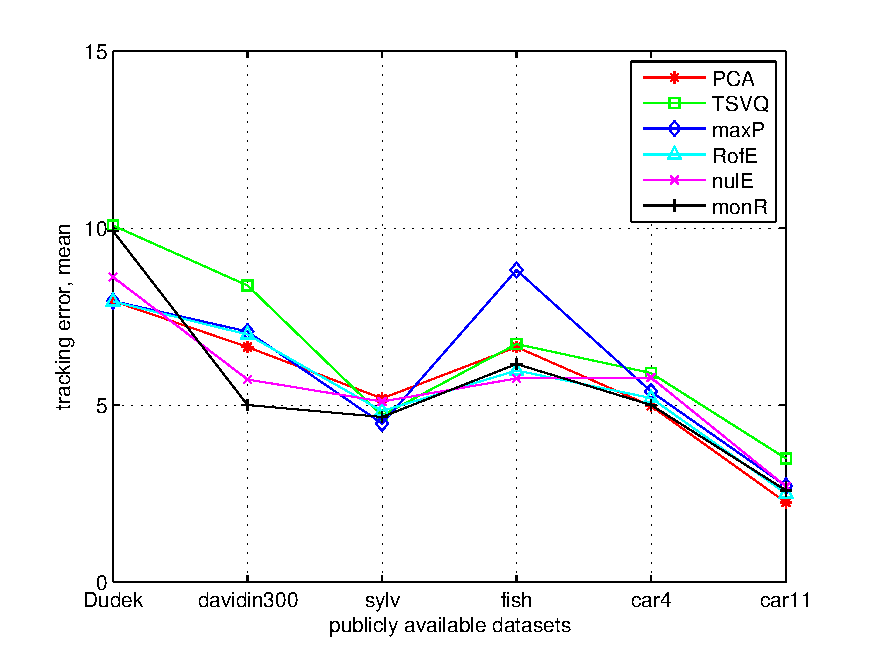
\includegraphics[width=0.47\textwidth]{temp/results_final_2a_mean.pdf}\label{fig:results_final_2a_mean}}
								\subfigure[]{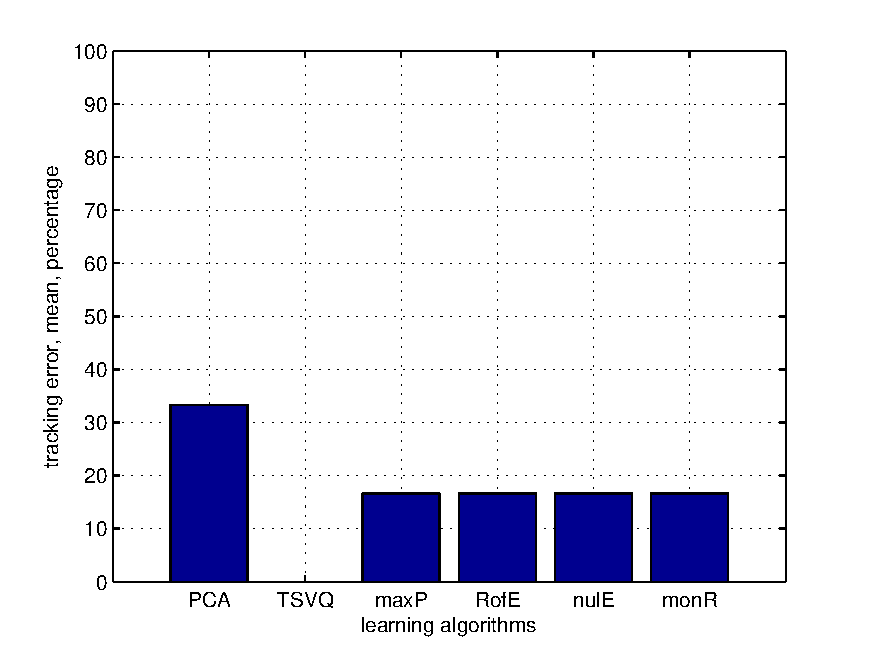
\includegraphics[width=0.47\textwidth]{temp/results_final_2b_mean_percent.pdf}\label{fig:results_final_2b_mean_percent}}
								\caption{Tracking results (2 of 5), comparison of mean tracking performance.}
								\label{fig:results_final_2_mean}
								\end{figure}


%\begin{enumerate}
%\item \underline{Continually increasing error}.  For Dudek and sylv, the error continues to increase from $Q=8$ to $Q=32$.
%\item \underline{Sharply decreasing, then sharply increasing error}. For davidin300 and fish, the error decreases from $Q=8$ to $Q=16$, and then increases from $Q=16$ to $Q=32$.   The tracking error at $Q=16$ is significantly lower than for $Q=8$ and $Q=32$.
%\item \underline{Mildly decreasing, then mildly increasing error}.  For car4 and car11, like for davidin300 and fish above, the error decreases from $Q=8$ to $Q=16$, and then increases from $Q=16$ to $Q=32$.  However, the drop and rise in error is not as steep.
%\item \underline{Highest error}.  The average error for the Dudek sequence is highest.  This is because this sequence contains more variation than all other sequences including temporary occlusions, expression changes, structured noise, lighting changes and pose changes.  
%\item \underline{Face tracking}.  
%\end{enumerate}

For the Dudek and davidin300 sequences which consist of tracking a face, we look at some related areas in the context of facial processing using PCA, 

\begin{enumerate}
\item \underline{Face reconstruction}.  It has been shown that 40 eigenfaces can be used to reconstruct a face with 3\% error~\cite{1987_JNL_Faces_Sirovich}.
\item \underline{Face recognition}.  Face recognition performance levels off at about 25 principal components, or 45 principal components if the first 3 principal components are dropped~\cite{1997_JNL_EigenVsFisherFaces_Bel}.  The reason for dropping 3 principal components is that~\cite{1992_THE_GeoPhoto_Shashua} showed that for a fixed viewpoint, images of a Lambertian surface\footnote{A Lambertian surface, or informally a matte surface, is a surface that has constant BRDF (bidirectional reflectance distribution function) $\rho(\theta_o, \phi_o, \theta_i, \phi_i)=\frac{L_o(x, \theta_o, \phi_o)}{L_i(x, \theta_i, \phi_i)\cos\theta_i d\omega}$, where the angles ($\theta_o, \phi_o$) define the outgoing light direction and angles ($\theta_i, \phi_i$) define the incoming light direction.  A surface illuminated by radiance $L_i(x, \theta_i, \phi_i)$ coming in from a differential region of solid angle $d\omega$ at angles $\theta_i, \phi_i$ receives irradiance $L_i(x, \theta_i, \phi_i)\cos\theta_i d\omega$.  Irradiance is measured in $\mathrm{W/m^2}$, while the solid angle $d\omega$ is measured in steridians, sr.  The unit of BRDF is therefore $\mathrm{sr^{-1}}$~\cite{2002_BOOK_CV_Forsyth}.} under varying lighting conditions lie in a 3D linear subspace of the high-dimensional image space.
\item \underline{Accounting for lighting changes in face recognition}.  As mentioned above, the first 3 principal components account for lighting changes in faces.  However, these components are unlikely to only account for lighting variation and removing them may result in loss of important information~\cite{1997_JNL_EigenVsFisherFaces_Bel}.
\end{enumerate}

								\begin{figure}[t]
								\centering
								\begin{tabular}{|l|c|c|c|c|c|c|}
\hline
&\textbf{PCA}&\textbf{TSVQ}&\textbf{maxP}&\textbf{RofE}&\textbf{nulE}&\textbf{monR}\\\hline
\textbf{Dudek}&7.81&8.62&7.78&7.11&9.65&11.81\\\hline
\textbf{davidin300}&4.60&12.88&6.84&9.02&7.17&50.00\\\hline
\textbf{sylv}&5.47&4.70&4.00&4.12&4.81&4.31\\\hline
\textbf{fish}&2.17&10.07&11.50&2.96&4.03&2.89\\\hline
\textbf{car4}&4.60&5.11&4.67&4.93&5.28&5.07\\\hline
\textbf{car11}&2.13&2.21&2.17&2.47&2.59&2.47\\\hline
\textbf{ \% best}&66.67&0.00&16.67&16.67&0.00&0.00\\\hline
\end{tabular}

								\subfigure[]{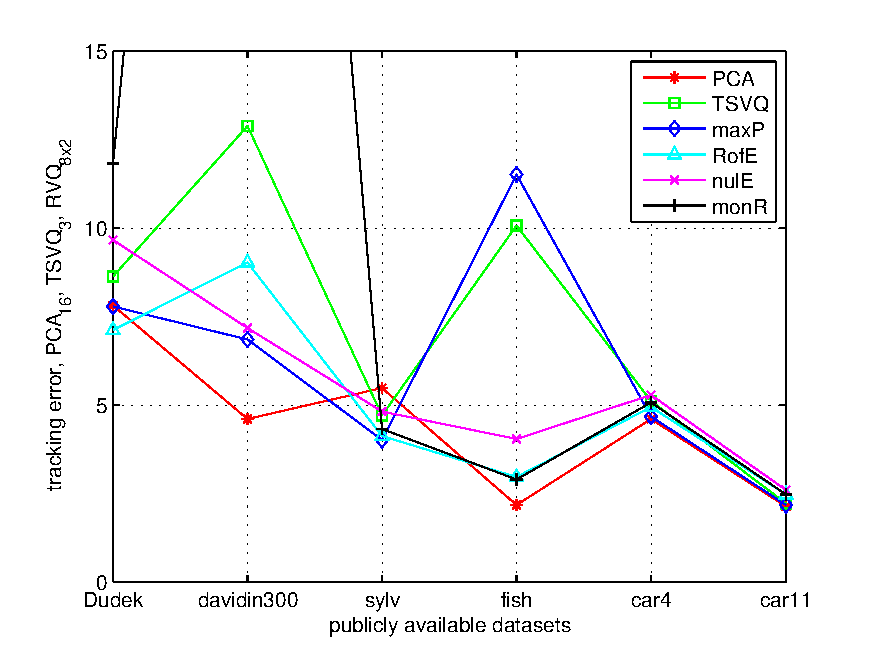
\includegraphics[width=0.47\textwidth]{temp/results_final_3a_16.pdf}\label{fig:results_final_3a_16}}
								\subfigure[]{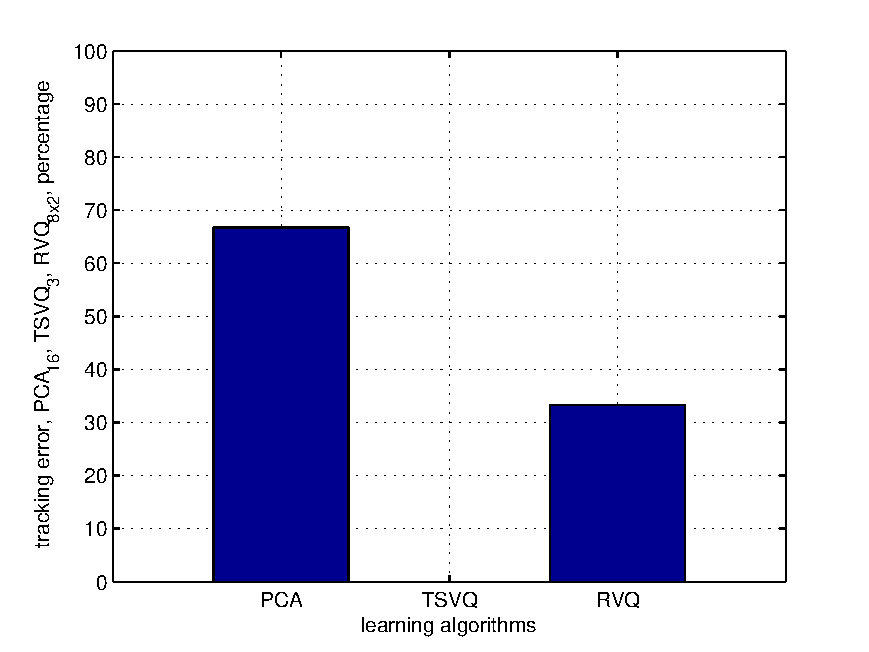
\includegraphics[width=0.47\textwidth]{temp/results_final_3b_16_percent.pdf}\label{fig:results_final_3b_16_percent}}
								\caption{Tracking results (3 of 5), comparison of tracking performance if 16 eigenvectors/code-vectors are stored in memory.}
								\label{fig:results_final_3_16}
								\end{figure}

Given these observations in related areas of facial processing, we do not remove any principal components.  However, unlike the face recognition case, our tracking performance does not keep increasing till 20 or more eigenvectors.  An important difference in tracking applications however is that face alignment is noisy.  It appears that in the Dudek and davidin300 sequences which have large pose changes, the first few eigenvectors are able to capture the linear dependencies in the slightly shifted faces.  After that, the later eigenvectors explain the residual noise.  This can lead to decreased tracking performance since reconstructions using an eigenspace that partially explains noise will be noisy.  Noisy reconstructions will get inaccurate DFFS (distance-from-feature-space) scores, which in turn will cause incorrect weighting for particle filter candidates in the tracking process.  This will lead to larger tracking error.

								\begin{figure}[t]
								\centering
								\begin{tabular}{|l|c|c|c|c|c|c|}
\hline
&\textbf{PCA}&\textbf{TSVQ}&\textbf{maxP}&\textbf{RofE}&\textbf{nulE}&\textbf{monR}\\\hline
\textbf{Dudek}&8.54&11.87&7.92&8.43&8.19&9.17\\\hline
\textbf{davidin300}&6.93&6.29&4.47&6.21&5.35&5.83\\\hline
\textbf{sylv}&5.72&4.80&4.68&5.54&5.74&4.58\\\hline
\textbf{fish}&7.98&4.59&2.78&12.22&2.48&3.62\\\hline
\textbf{car4}&5.52&6.79&6.38&5.14&5.84&5.18\\\hline
\textbf{car11}&2.39&5.28&2.36&2.33&2.52&2.72\\\hline
\textbf{ \% best}&0.00&0.00&33.33&33.33&16.67&16.67\\\hline
\end{tabular}

								\subfigure[]{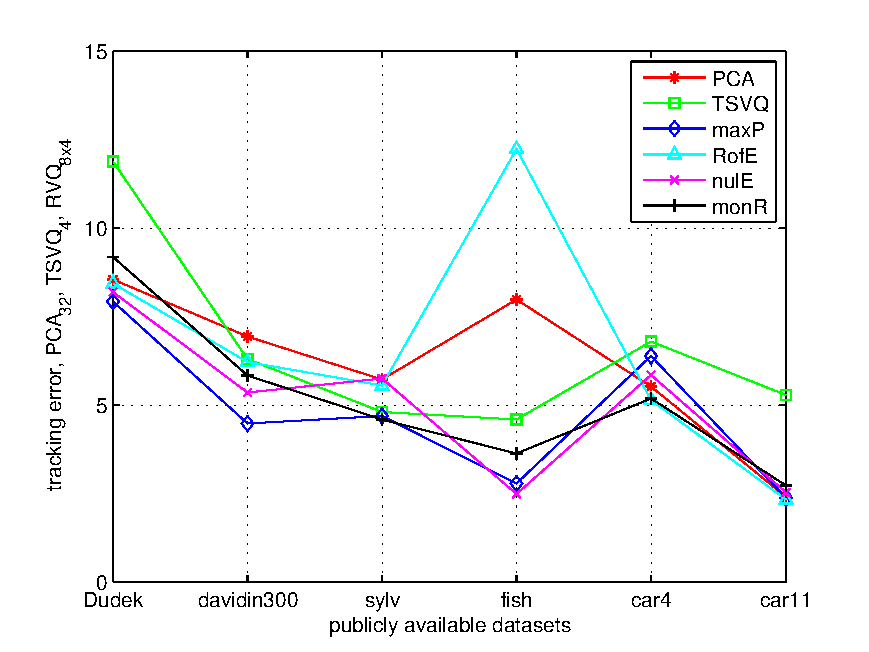
\includegraphics[width=0.47\textwidth]{temp/results_final_4a_32.pdf}\label{fig:results_final_4a_32}}
								\subfigure[]{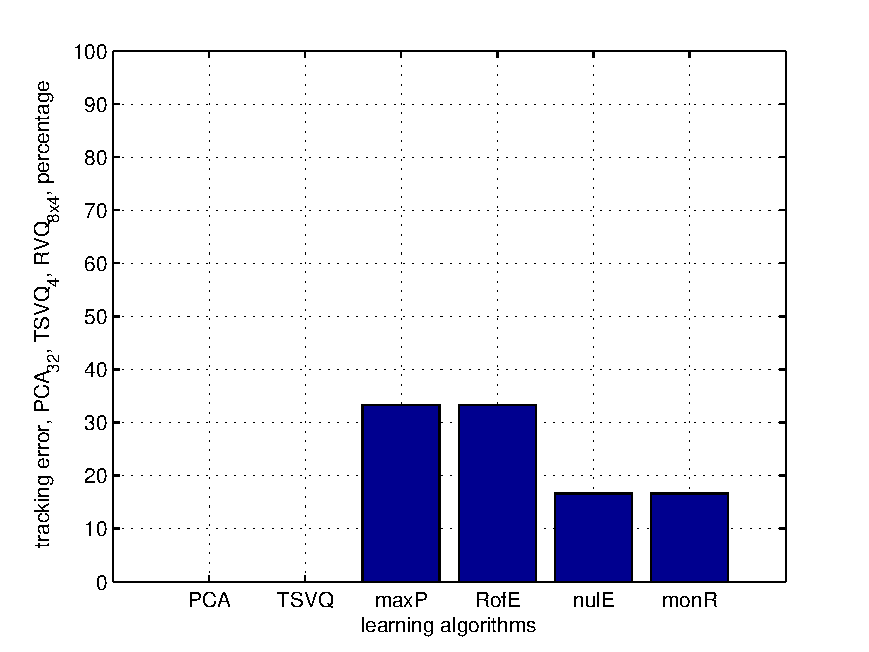
\includegraphics[width=0.47\textwidth]{temp/results_final_4b_32_percent.pdf}\label{fig:results_final_4b_32_percent}}
								\caption{Tracking results (4 of 5), comparison of tracking performance if 32 eigenvectors/code-vectors are stored in memory.}
								\label{fig:results_final_4_32}
								\end{figure}

%=========================
\section{Results}
%=========================
Our final tracking results are plotted in 5 figures, Figures~\ref{fig:results_final_1_best}, \ref{fig:results_final_2_mean}, \ref{fig:results_final_3_16}, \ref{fig:results_final_4_32} and~\ref{fig:results_final_5_configs}.  These plots are based entirely on detailed plots in Figures~\ref{fig:results_final_pca_}, \ref{fig:results_final_tsvq}, \ref{fig:results_final_maxP}, \ref{fig:results_final_RofE} \ref{fig:results_final_nulE} and \ref{fig:results_final_monR} in Appendix~\ref{App:tracking_error_plots} for PCA, TSVQ, maxP, RofE, nulE and monR respectively.

We start with Figure~\ref{fig:results_final_1_best}.  In this figure, we plot best possible tracking performance for each algorithm.  For PCA, this means the best possible performance attained for each of the datasets for $Q$=8, 16 and 32.  For TSVQ, best possible performance for each dataset is over $P$=3, 4 and 5.  For maxP, RofE, nulE and monR, best possible performance for each dataset is over 8x2, 8x4 and 8x8.  The reason for plotting performance for each dataset separately is that each dataset represents a different distribution and we would like to gauge performance for each algorithm over the different distributions.  We see that performance for PCA and all 4 RVQ based algorithms is very close while TSVQ tracking error is highest in most cases.  

PCA performs best in the fish, car4 and car11 sequences while RVQ performs best in the remaining three datasets, Dudek, davidin300 and sylv.  TSVQ does not perform best in any sequence.  Note that the performance difference between PCA and RVQ in the car4 and car11 sequences is negligible.  Recall that car4 and car11 are relatively benign datasets with little variation in pose and lighting.  The fish sequence has sudden motion as well as sudden global lighting changes.   Since global lighting change induces linear correlation in the data, it makes sense that PCA does well in this sequence.  The reason is that global illumination moves the illuminated object within the modeled PCA subspace~\cite{1987_JNL_Faces_Sirovich}.  For a VQ based method such as RVQ or TSVQ, several codevectors would have to be dedicated to different lighting conditions to model all possible lighting changes.  

RVQ performs best over the Dudek, davidin300 and sylv sequences.  All 3 of these sequences have moderate lighting changes while Dudek and davidin300 have several forms of noise as discussed earlier.  For Dudek, RofE does best.  The reason is that in the presence of uncertainties, RofE holds tight to what has already been modeled and is resistant to accepting sudden changes in the underlying distribution.  It is therefore better able to handle blur and other forms of noise that did not exist in the training data.  On the other extreme is monR which greedily attempts to minimize reconstruction error.  Out of all RVQ methods, this method performs worse, but even then, not by much.  Second best performance is for maxP which is again not a greedy method.  Third best performance is for nulE which is also a greedy method but less so than monR.

								\begin{figure}[h!]
								\centering
								\subtable[PCA]{\begin{tabular}{|c|c|c|c|}
\hline
\textbf{8}&\textbf{16}&\textbf{32}&\textbf{mean}\\\hline
6.15&4.46&6.18&5.60\\\hline
\end{tabular}
}\hspace{0.2in}
								\subtable[TSVQ]{\begin{tabular}{|c|c|c|c|}
\hline
\textbf{3}&\textbf{4}&\textbf{5}&\textbf{mean}\\\hline
7.26&6.60&5.74&6.54\\\hline
\end{tabular}
}\\
								\subtable[maxP]{\begin{tabular}{|c|c|c|c|}
\hline
\textbf{8x2}&\textbf{8x4}&\textbf{8x8}&\textbf{mean}\\\hline
6.16&4.76&7.25&6.06\\\hline
\end{tabular}
}\hspace{0.2in}
								\subtable[RofE]{\begin{tabular}{|c|c|c|c|}
\hline
\textbf{8x2}&\textbf{8x4}&\textbf{8x8}&\textbf{mean}\\\hline
5.10&6.64&4.94&5.56\\\hline
\end{tabular}
}\\
								\subtable[nulE]{\begin{tabular}{|c|c|c|c|}
\hline
\textbf{8x2}&\textbf{8x4}&\textbf{8x8}&\textbf{mean}\\\hline
5.59&5.02&6.20&5.60\\\hline
\end{tabular}
}\hspace{0.2in}
								\subtable[monR]{\begin{tabular}{|c|c|c|c|}
\hline
\textbf{8x2}&\textbf{8x4}&\textbf{8x8}&\textbf{mean}\\\hline
5.31&5.18&6.19&5.56\\\hline
\end{tabular}
}\\
								\subfigure[PCA]{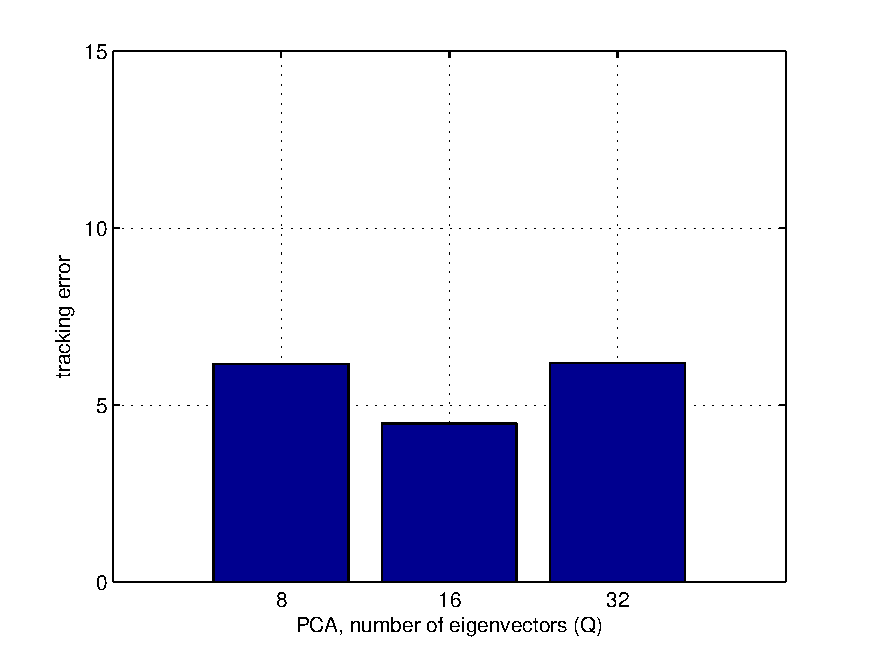
\includegraphics[width=0.3\textwidth]{temp/results_final_5a_pca_.pdf}\label{fig:results_final_5a_pca_}}
								\subfigure[TSVQ]{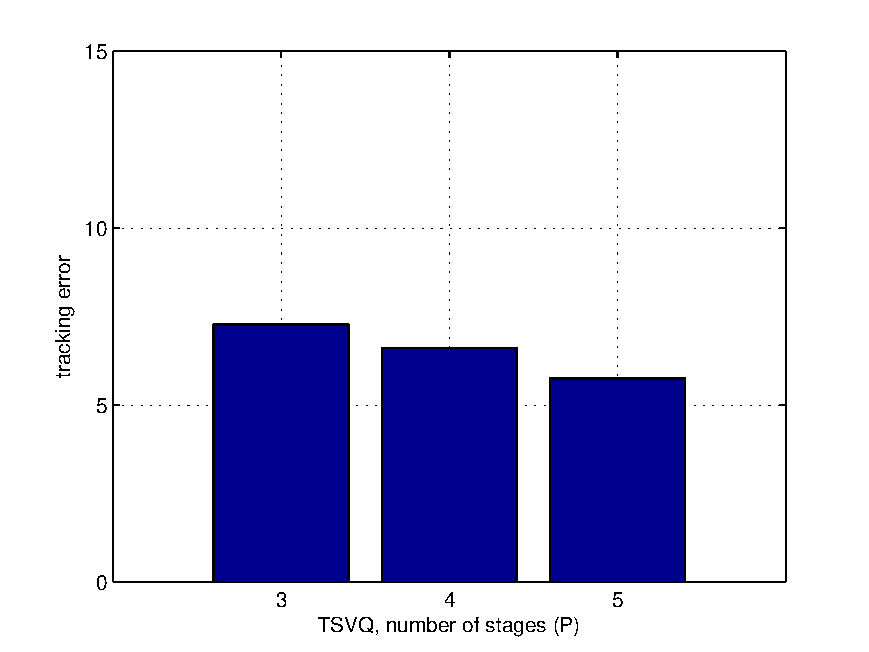
\includegraphics[width=0.3\textwidth]{temp/results_final_5b_tsvq.pdf}\label{fig:results_final_5b}}
								\subfigure[maxP]{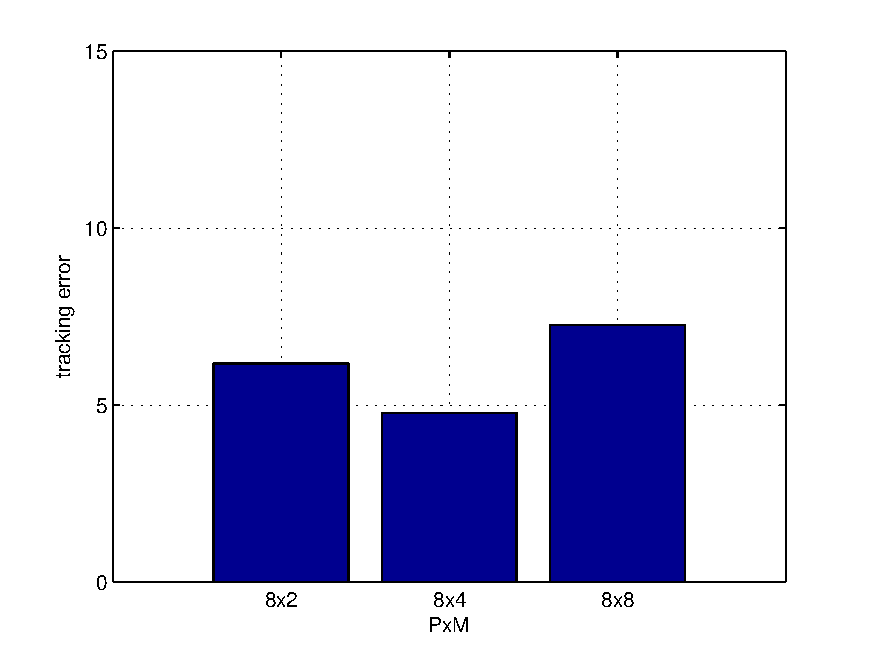
\includegraphics[width=0.3\textwidth]{temp/results_final_5c_maxP.pdf}\label{fig:results_final_5c}}
								\subfigure[RofE]{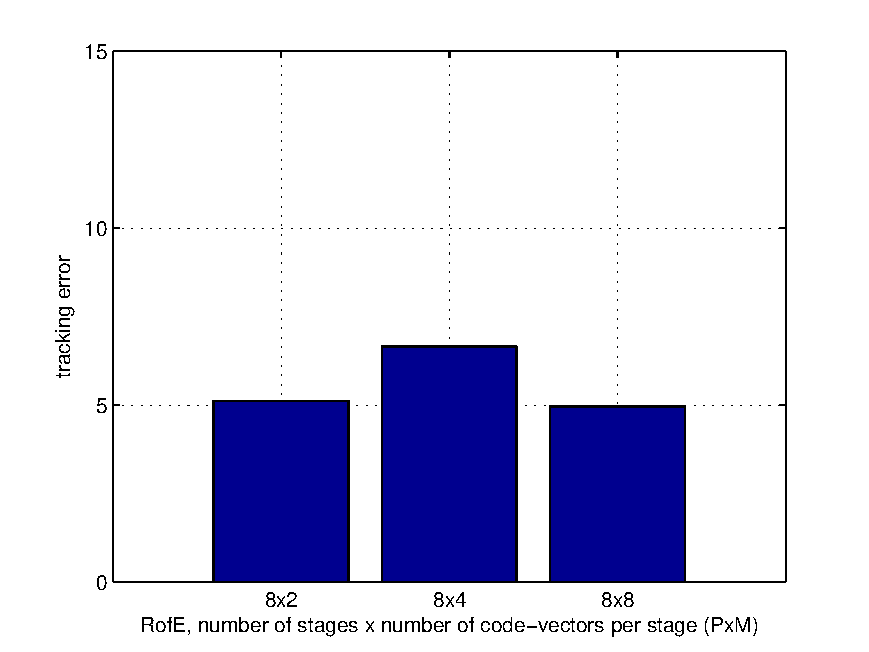
\includegraphics[width=0.3\textwidth]{temp/results_final_5d_RofE.pdf}\label{fig:results_final_5d}}
								\subfigure[nulE]{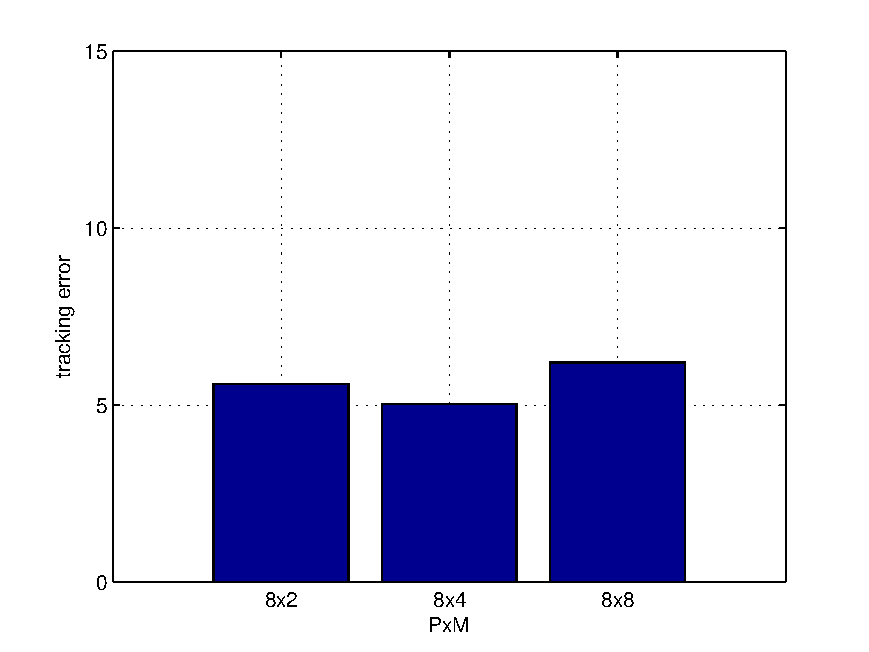
\includegraphics[width=0.3\textwidth]{temp/results_final_5e_nulE.pdf}\label{fig:results_final_5e}}
								\subfigure[monR]{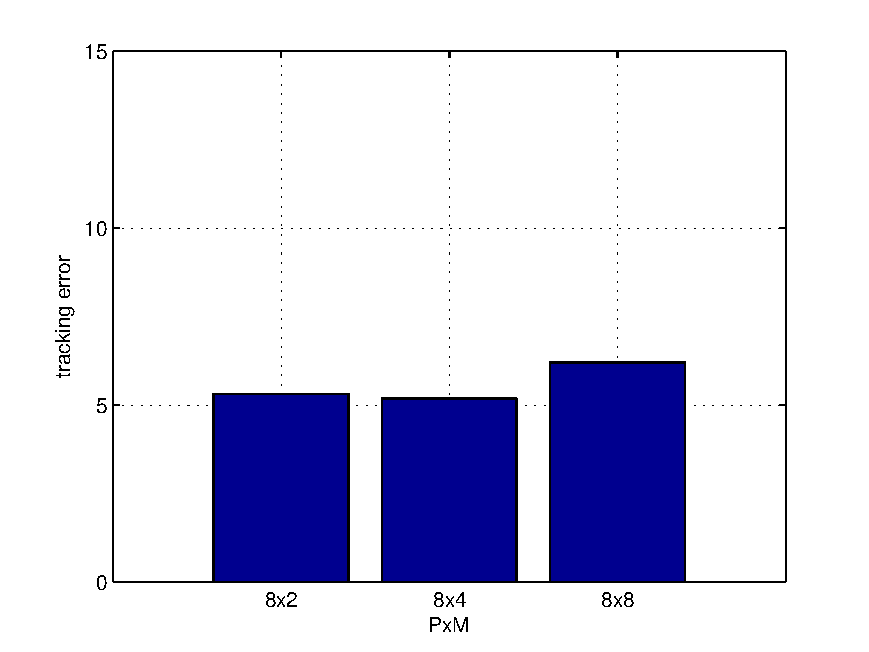
\includegraphics[width=0.3\textwidth]{temp/results_final_5f_monR.pdf}\label{fig:results_final_5f}}
								\caption{Tracking results (5 of 5), comparison of tracking performance as parameters for each algorithm are varied.}
								\label{fig:results_final_5_configs}
								\end{figure}


We now turn to Figure~\ref{fig:results_final_2_mean}.  In this figure, mean performance over all configurations is shown.  It may be noted that monR loses track in one instance.  That instance is not factored into the means since it is not clear how penalize a lost track when performing mean computations.  Here, we see that RVQ performs best 66.7\% of the time.  This time, in addition to Dudek, davindin300 and sylv, RVQ performs better than PCA in the fish sequence as well.  The reason for this is that PCA is unable to track the fish sequence well when it has too few, i.e., 8 eigenvectors or when it has too many, i.e., 32 eigenvectors.  In the 8 eigenvector case, the subspace does not have enough dimensions to model lighting changes well.  Even though it has been shown, as mentioned earlier, that only 3 eigenvectors are needed to model lighting changes~\cite{1987_JNL_Faces_Sirovich}, in practice this does not hold due to shadowing and specularities~\cite{1997_JNL_EigenVsFisherFaces_Bel}.  For too many eigenvectors, over-fitting is an issue as mentioned in an earlier report.  For $Q=16$, PCA performs best and that is why it had best possible performance.  However, when it comes to means, all 4 RVQ configurations are able to outperform PCA in mean performance.

In Figures~\ref{fig:results_final_3_16} and~\ref{fig:results_final_4_32}, we hold the number of eigenvectors for PCA or codevectors for TSVQ and RVQ constant at 16 and 32 respectively\footnote{This is 15 and 31 actually for TSVQ but we ignore this slight difference.}.  In these figures, we see that PCA outperforms RVQ for 16 vectors but RVQ completely outperforms PCA for 32 vectors.  For a given memory cost, and therefore for a given rate, RVQ overall outperforms PCA.  

Finally, in Figure~\ref{fig:results_final_5_configs}, we plot tracking performance for each algoritm separately for its different configurations.  For 3 configurations per algorithm, $Q$=8, 16, 32 for PCA, $P$=3, 4, 5 for TSVQ and $PxM$ = 8x2, 8x4, 8x8 for RVQ, there are 4 possible outcomes listed below.  Of these, the first 3 are to be expected.  The fourth however requires further scrutiny.

\begin{enumerate}
\item \underline{Monotonically increasing error.}  This would mean that the degrees of freedom (DoF) in the learning algorithm, such as PCA, TSVQ or RVQ, model the underlying distribution well with low DoFs and adding DoFs is leading to over-generalization.  We do not see this performance in any case since we start with low DoFs.  We got an initial estimate of how many DoFs to use using our experiments on appearance modeling that have mentioned in a previous report.
\item \underline{Monotonically decreasing error.}  This happens for TSVQ.  This means that adding more stages to TSVQ may increase performance.  In our case, we use 3, 4 and 5 stages to keep the DoFs in TSVQ close to the DoFs for RVQ and PCA.
\item \underline{Decreasing error followed by increasing error.}  We see this performance for PCA, maxP, nulE and monR.  This is a sign that the correct number of DoFs were chosen and that when error is minimum, the algorithm now has enough capacity to model the underlying distribution, but without over-fitting.
\item \underline{Increasing error followed by decreasing error.}  We see this in one case, RofE, and in some cases in TSVQ in Figure~\ref{fig:results_final_tsvq}.  To see this, consider the example of $K$=2, 4 and 8 code-vectors in $\mathbb{R}$ uniformly spaced on the inteval [0,7].  For $K$=2, the code-vectors are 2.33 and 4.66.  For the $K$=4 case, the code-vectors are 1.4, 2.8, 4.2 and 5.6.  For the $K$=8 case, the code-vectors are $\{0, 1, 2, 3, \ldots, 7\}$.  In regions around 2.33 and 4.6, there are certain contiguous regions where the reconstruction error is greatest for $K$=4.  This shows that although in general, one would not expect reconstruction error, and therefore tracking error to be lowest for an intermediate number of code-vectors $K$, it is possible for a test vector to score highest error for an intermediate $K$.  If this occurs at a point in the tracking process where the target is moving quickly for instance, then a wrong decision can cause tracking error to increase.  In certain cases, it may not be possible to recover from this wrong decision.  See Figures~\ref{fig:results_TSVQ_Dudek_errors}, \ref{fig:results_TSVQ_Dudek_FN10} and \ref{fig:results_TSVQ_Dudek_FN457} in Appendix~\ref{App:TSVQ_Dudek_example} for an example of such a scenario for TSVQ tracking.


\end{enumerate}

%
%For PCA, on average, $Q=16$ produces the lowest tracking error.  On average, the tracking error decreases from $Q=8$ to $Q=16$, and then increases from $Q=16$ to $Q=32$.  It appears that the number of eigenvectors required to capture the linear correlation in these datasets is between 16 and 32, but closer to 16.   






%=========================
\section{Conclusions}
%=========================
Based on the experiments conducted in this report, we draw the following conclusions:

\begin{enumerate}
\item \underline{Performance comparison}.  We chose three metrics to compare PCA, TSVQ and RVQ.  A fourth metric is added which counts number of lost drifts.
\begin{enumerate}
\item \underline{Best possible performance}.  PCA and RVQ performed best in half the times each.  TSVQ never performed best.  However, of the 3 times that PCA performed best, in 2 cases, the performance difference was not significantly better than RVQ.  Moreover, and perhaps more importantly, RVQ performed best in the two most challenging datasets, Dudek and davidin300 since they both have multiple sources of noise.
\item \underline{Best mean performance}.  Here, RVQ performed best in twice the number of scenarios as PCA.  TSVQ had the worst mean performance.
\item \underline{Memory cost=16 vectors}.  Here PCA performed best in twice the number of scenarios as RVQ .
\item \underline{Memory cost=32 vectors}.  Here RVQ completely outperformed PCA and TSVQ.  This is understandable since the capacity of RVQ to explain an underlying distribution grows exponentially as $M^P$.  Moreover, we have used $M=2, 4, 8$ ensuring that we do not increase our VC dimension too much so as to start over-fitting.
\item \underline{Lost tracks}.  There was only one lost track for monR.  This is understandable since monR is a greedy approach.  The lost track was in davidin300 which is a challenging dataset.
\end{enumerate}

\item \underline{Target alignment}.  In tracking scenarios, accurate alignment of targets is difficult.  In the case of PCA for instance, it has been mentioned earlier that between 25 to 45 eigenvectors can be used for accurate face reconstruction~\cite{1997_JNL_EigenVsFisherFaces_Bel}.  In our case, for the Dudek sequence that has faces, PCA with 16 eigenvectors was able to capture the linear dependence between slightly shifted versions of the same target since slight shifts still preserve correlation.  However, as the number of eigenvectors increased further, the additional eigenvectors explained noise in the data.  This scenario can lead to noisy reconstructions and subsequent noisy weighting for target candidates.  When the noisy target candidate that is best explained by the PCA subspace is then added to the training set to update the PCA subspace, the resulting subspace will be noisy which will further increase the chances of noisy reconstructions.  
\end{enumerate}

Overall, PCA and RVQ outperform TSVQ completely.  Between PCA and RVQ, RVQ outperforms PCA in more areas.  In a tracking scenario, it is desirable to try different algorithms to get a feel for the dynamics of the underlying distribution.  Specifically, it is desired to understand how many DoFs are needed for a given algorithm to explain the distribution.  Our experiments show that averaged over all distributions and over all algorithms and their parameters, 8x4 RofE performs the best.  The reason is that 8x4 has a moderate VC dimension and that RofE is resistant to noise since it will penalize candidate snippets that have not appeared before.  In this sense, it allows the RVQ codebook to adapt gradually to the changing underlying distribution as tracking progresses over time.


%
%The reason for the decrease in tracking error is that a certain number of eigenvectors are needed to capture the linear correlations in the data.  A subsequent increase in tracking error, as discussed earlier, appears to be related to the difficulty in correctly aligning the targets which causes later PCA eigenvectors to explain noise.



\appendix
%==========================
\clearpage
\newpage
\section{Datasets}
\label{App:dataset_snapshots}
%==========================

									\begin{figure}[h!]
									\centering\subfigure[Dudek.]{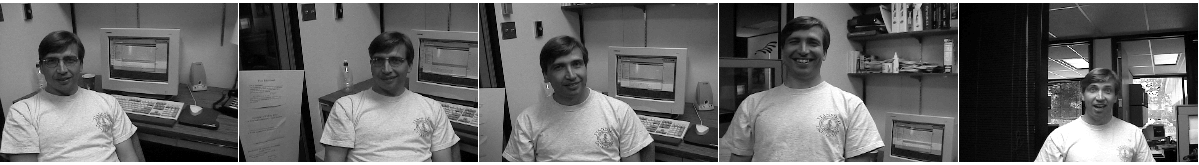
\includegraphics[height=0.95in]{thesis/seq_1_Dudek.png}\label{fig:trk_pca_1a}}
									\subfigure[Davidin300.]{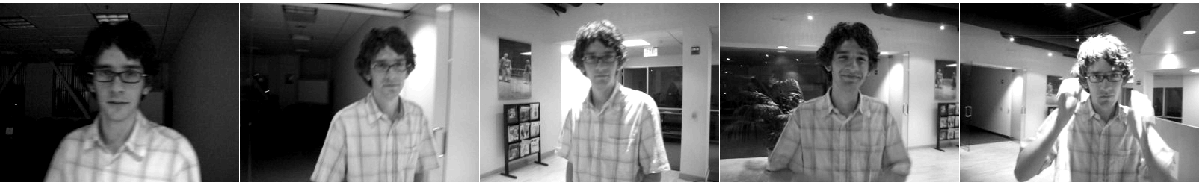
\includegraphics[height=0.95in]{thesis/seq_2_davidin300.png}\label{fig:trk_pca_1b}}
									\subfigure[Sylv.]{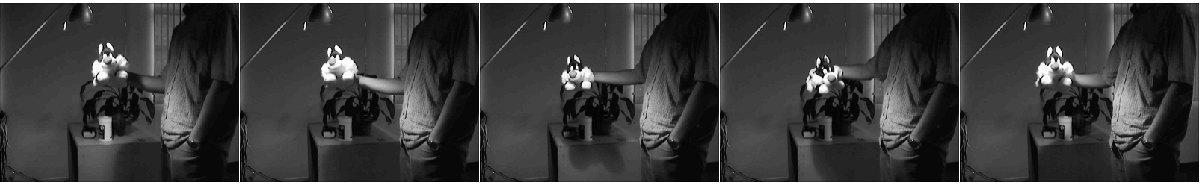
\includegraphics[height=0.95in]{thesis/seq_3_sylv.png}\label{fig:trk_pca_1c}}
									\subfigure[Fish.]{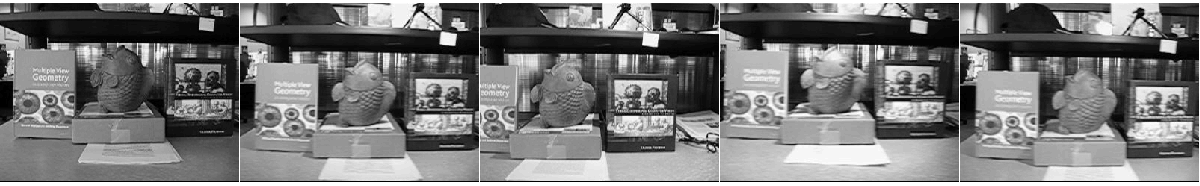
\includegraphics[height=0.95in]{thesis/seq_5_fish.png}\label{fig:trk_pca_1d}}
									\subfigure[Car4.]{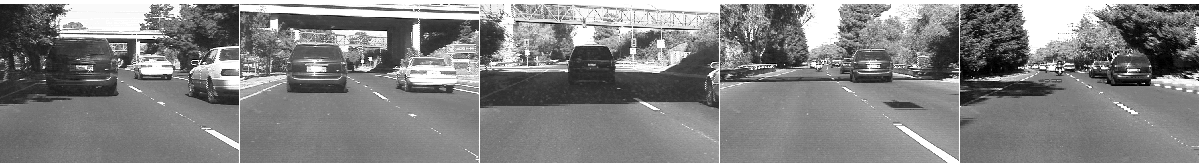
\includegraphics[height=0.95in]{thesis/seq_6_car4.png}\label{fig:trk_pca_1d}}
									\subfigure[Car11.]{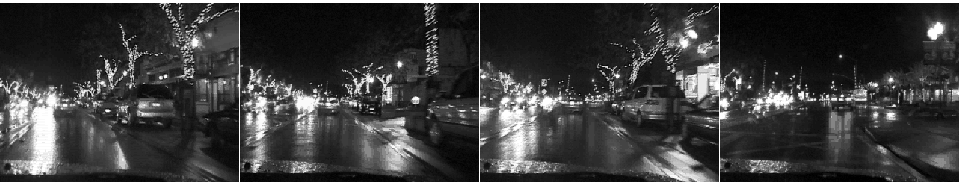
\includegraphics[height=0.95in]{thesis/seq_7_car11.png}\label{fig:trk_pca_1d}}
									\caption{Publicly available tracking sequences downloadable from~\cite{2008_JNL_subspaceTRK_Ross}.}
									\label{fig:trk_sequences}
									\end{figure}


%==========================
\clearpage
\newpage
\section{Tracking error plots}
\label{App:tracking_error_plots}
%==========================
The following 6 pages contain tracking error plots for PCA, TSVQ, maxP, RofE, nulE and monR based trackers respectively.

%----------------------------------------------------
\clearpage
\newpage
\subsection{PCA}
%----------------------------------------------------
\begin{figure}[h!]
\centering
\begin{tabular}{|l|c|c|c|}
\hline
&\textbf{Q=8}&\textbf{Q=16}&\textbf{Q=32}\\\hline
\textbf{1. Dudek}&7.44&7.81&8.54\\\hline
\textbf{2. davidin300}&8.36&4.60&6.93\\\hline
\textbf{3. sylv}&4.34&5.47&5.72\\\hline
\textbf{4. fish}&9.75&2.17&7.98\\\hline
\textbf{5. car4}&4.79&4.60&5.52\\\hline
\textbf{6. car11}&2.21&2.13&2.39\\\hline
\textbf{mean}&6.15&4.46&6.18\\\hline
\end{tabular}
\\
\subfigure[]{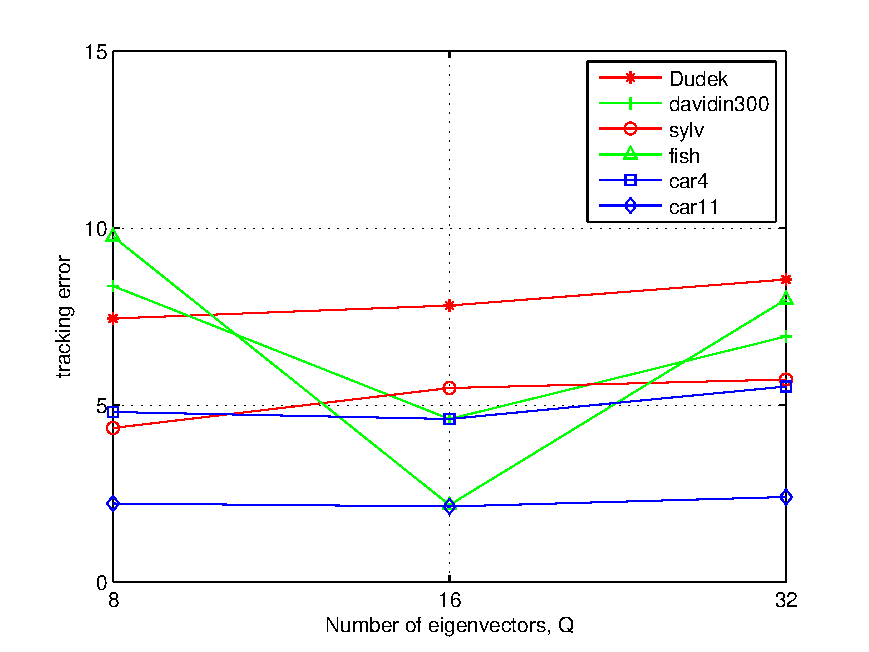
\includegraphics[width=0.45\textwidth]{temp/results_final_pca__a.pdf}\label{fig:results_final_pca__a}}
\subfigure[]{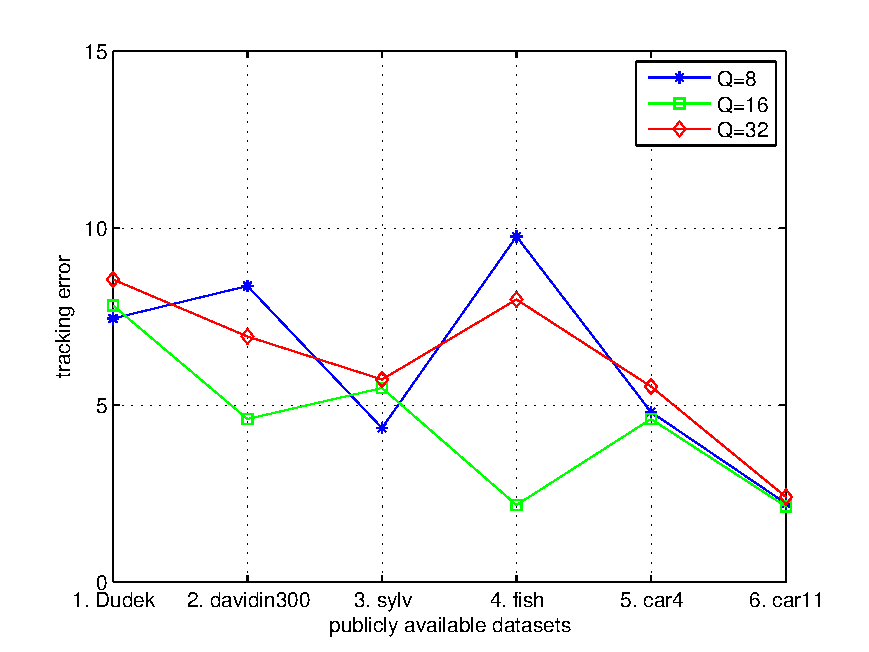
\includegraphics[width=0.45\textwidth]{temp/results_final_pca__b.pdf}\label{fig:results_final_pca__b}}
\subfigure[]{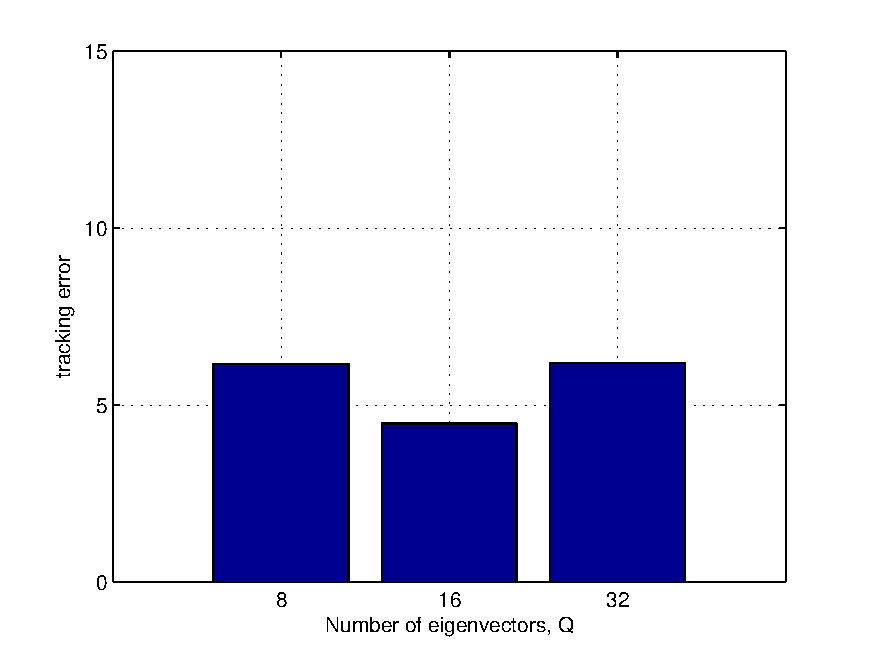
\includegraphics[width=0.45\textwidth]{temp/results_final_pca__c.pdf}\label{fig:results_final_pca__c}}
\subfigure[]{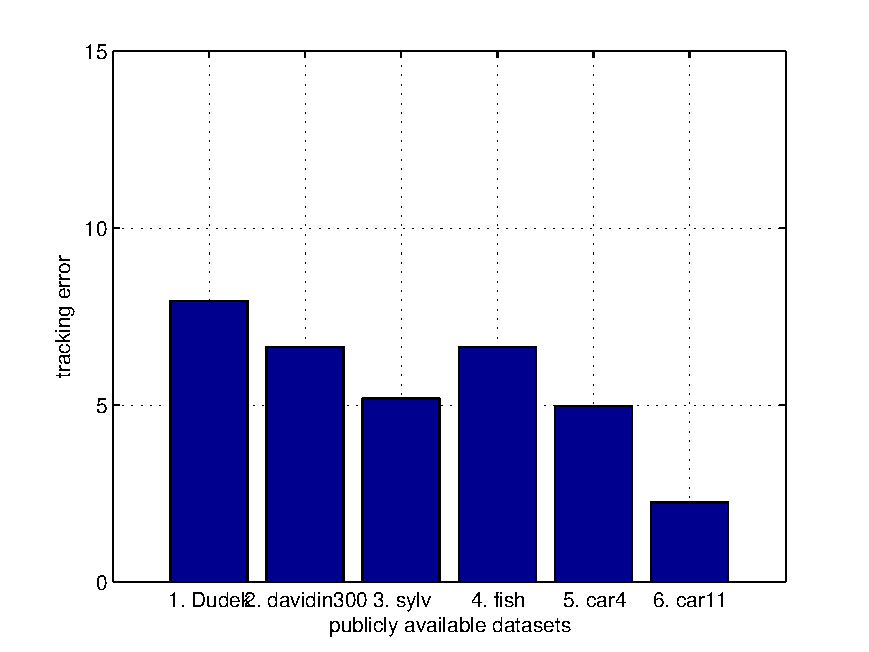
\includegraphics[width=0.45\textwidth]{temp/results_final_pca__d.pdf}\label{fig:results_final_pca__d}}
\caption{Tracking error for PCA based tracking for different number of eigenvectors $Q$ for 6 different publicly available datasets.}
\label{fig:results_final_pca_}
\end{figure}

%----------------------------------------------------
\clearpage
\newpage
\subsection{TSVQ}
%----------------------------------------------------
\begin{figure}[h!]
\centering
\begin{tabular}{|l|c|c|c|}
\hline
&\textbf{P=3}&\textbf{P=4}&\textbf{P=5}\\\hline
\textbf{Dudek}&8.62&11.87&9.71\\\hline
\textbf{davidin300}&12.88&6.29&5.93\\\hline
\textbf{sylv}&4.70&4.80&4.61\\\hline
\textbf{fish}&10.07&4.59&5.47\\\hline
\textbf{car4}&5.11&6.79&5.80\\\hline
\textbf{car11}&2.21&5.28&2.94\\\hline
\end{tabular}
\\
\subfigure[]{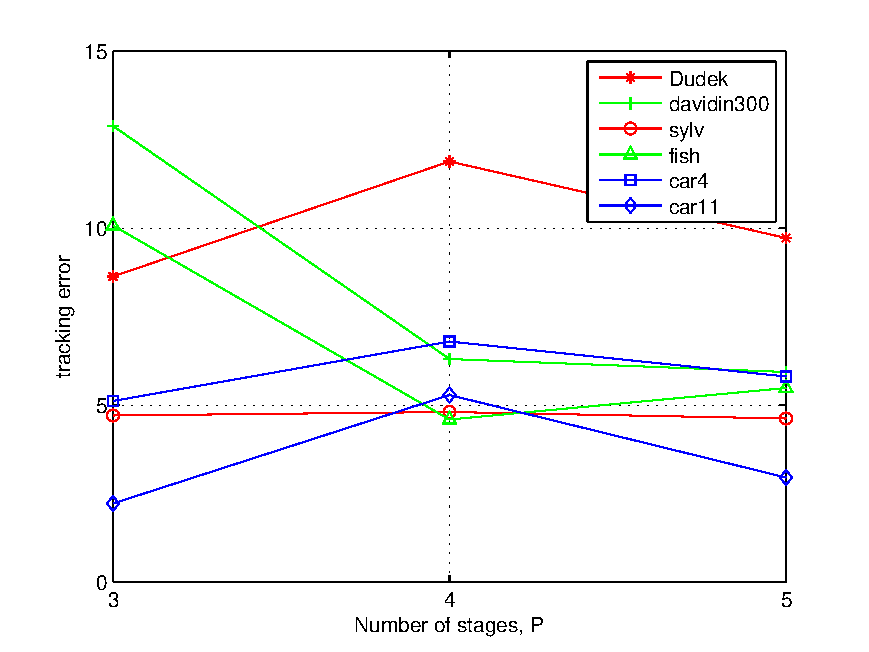
\includegraphics[width=0.45\textwidth]{temp/results_final_tsvq_a.pdf}\label{fig:results_final_tsvq_a}}
\subfigure[]{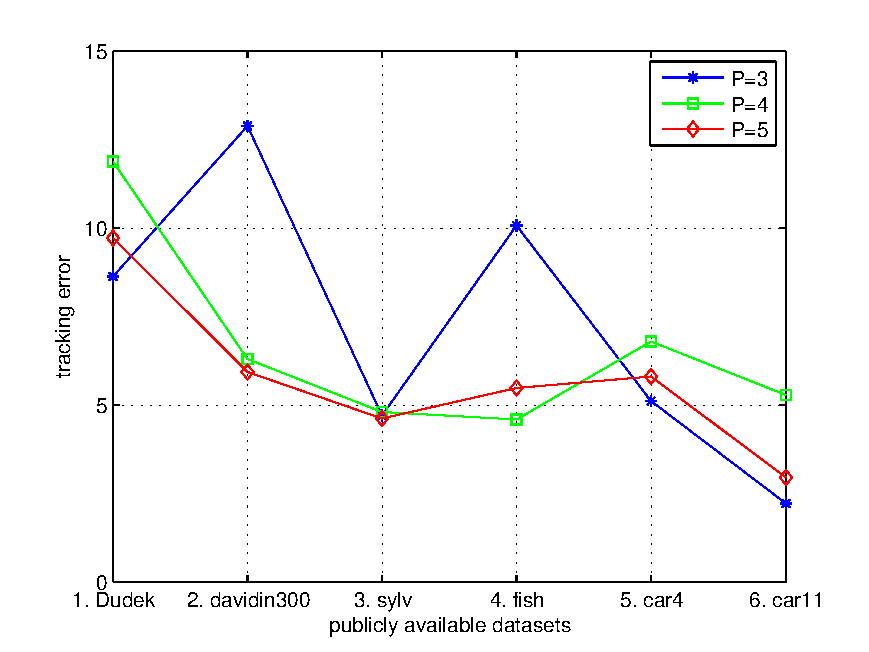
\includegraphics[width=0.45\textwidth]{temp/results_final_tsvq_b.pdf}\label{fig:results_final_tsvq_b}}
\subfigure[]{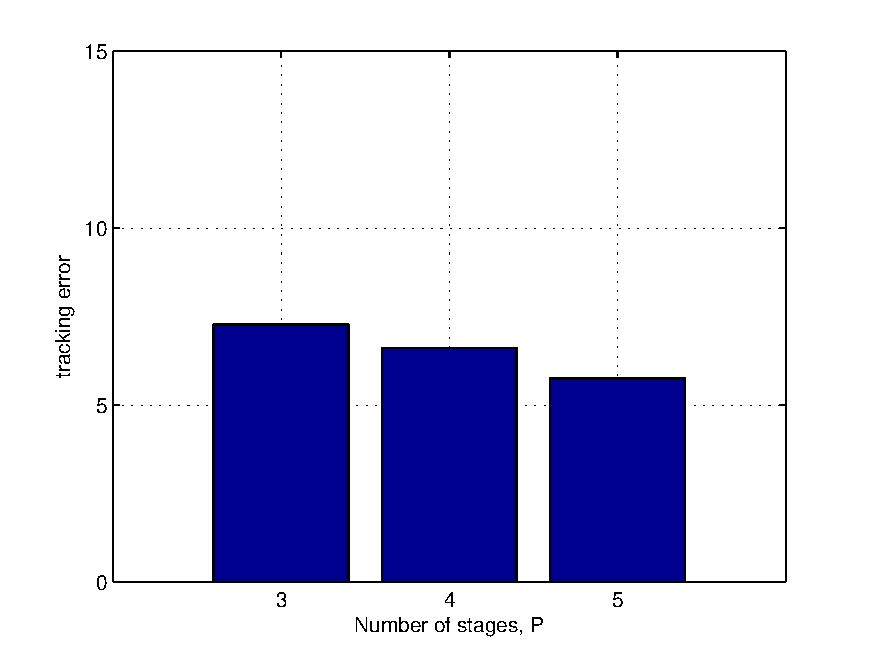
\includegraphics[width=0.45\textwidth]{temp/results_final_tsvq_c.pdf}\label{fig:results_final_tsvq_c}}
\subfigure[]{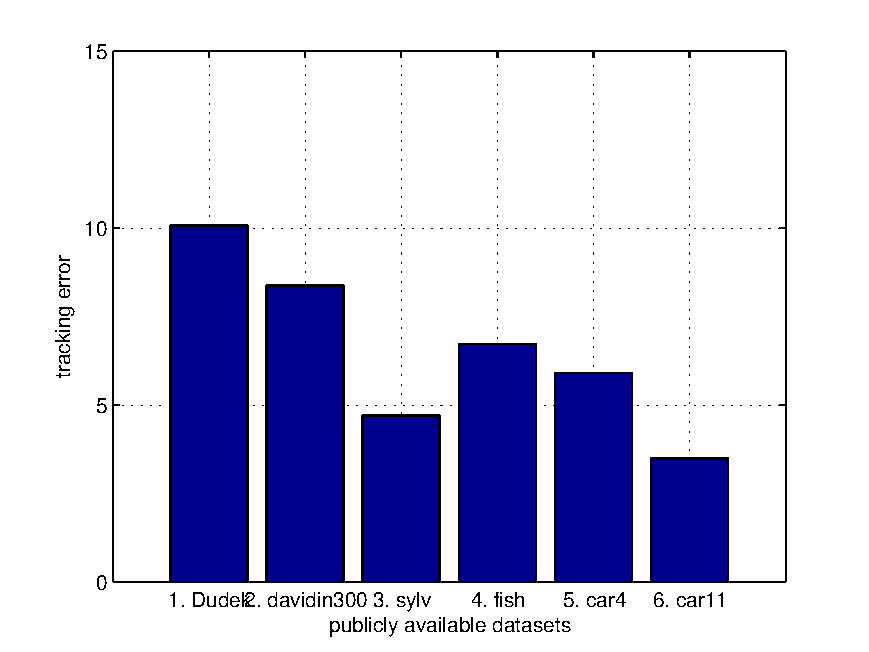
\includegraphics[width=0.45\textwidth]{temp/results_final_tsvq_d.pdf}\label{fig:results_final_tsvq_d}}
\caption{Tracking error for binary balanced-tree-TSVQ based tracking for different number of stages $P$ for 6 different publicly available datasets.}
\label{fig:results_final_tsvq}
\end{figure}


%----------------------------------------------------
\clearpage
\newpage
\subsection{maxP}
%----------------------------------------------------
\begin{figure}[h!]
\centering
\begin{tabular}{|l|c|c|c|}
\hline
&\textbf{PxM=8x2}&\textbf{PxM=8x4}&\textbf{PxM=8x8}\\\hline
\textbf{Dudek}&7.78&7.92&8.09\\\hline
\textbf{davidin300}&6.84&4.47&9.89\\\hline
\textbf{sylv}&4.00&4.68&4.72\\\hline
\textbf{fish}&11.50&2.78&12.15\\\hline
\textbf{car4}&4.67&6.38&5.09\\\hline
\textbf{car11}&2.17&2.36&3.57\\\hline
\end{tabular}
\\
\subfigure[]{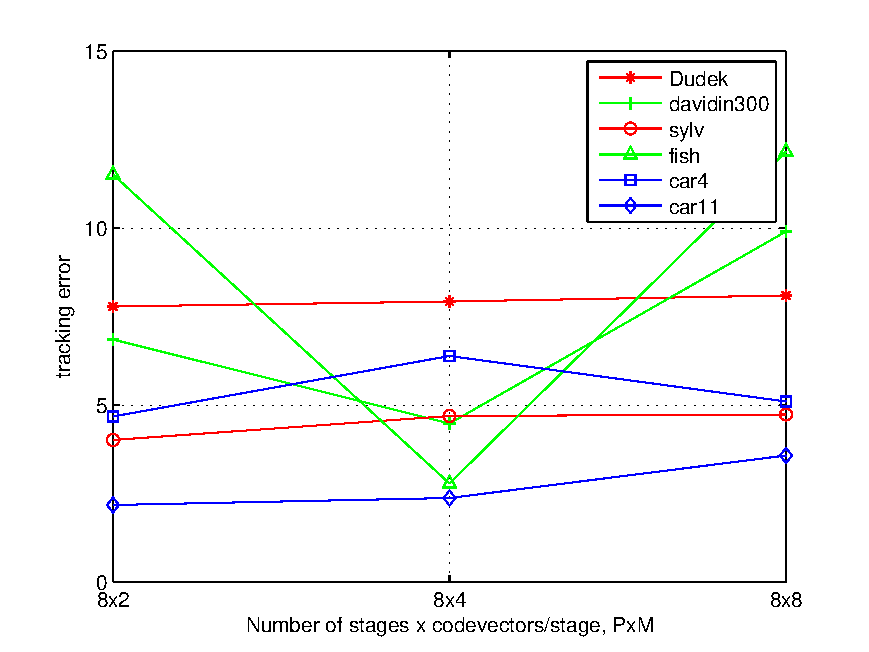
\includegraphics[width=0.45\textwidth]{temp/results_final_maxP_a.pdf}\label{fig:results_final_maxP_a}}
\subfigure[]{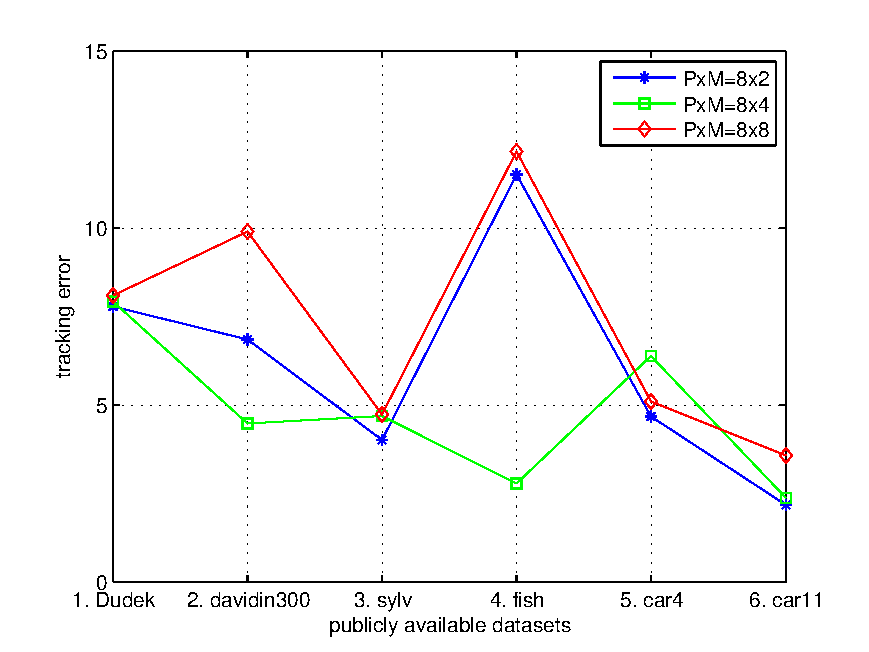
\includegraphics[width=0.45\textwidth]{temp/results_final_maxP_b.pdf}\label{fig:results_final_maxP_b}}
\subfigure[]{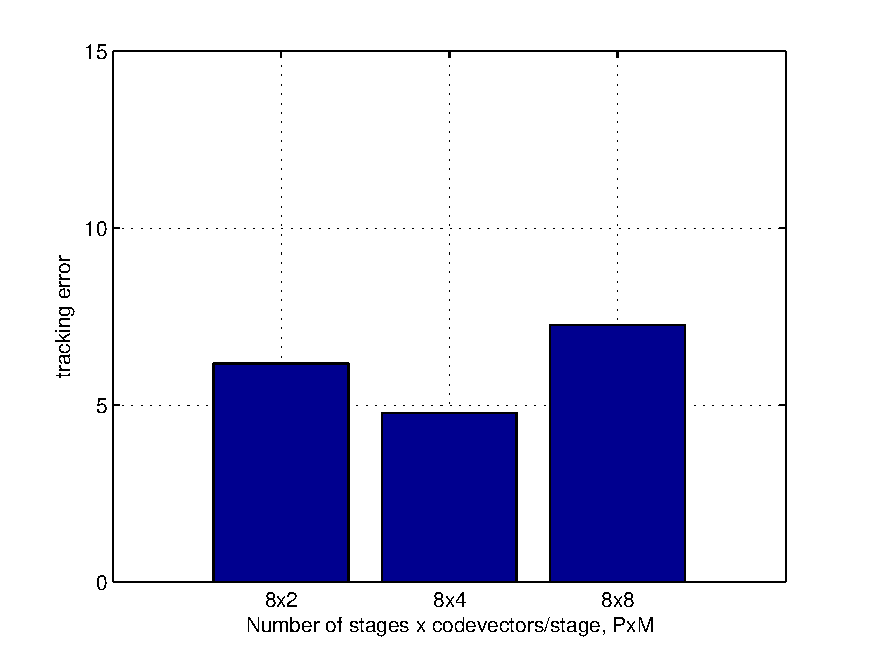
\includegraphics[width=0.45\textwidth]{temp/results_final_maxP_c.pdf}\label{fig:results_final_maxP_c}}
\subfigure[]{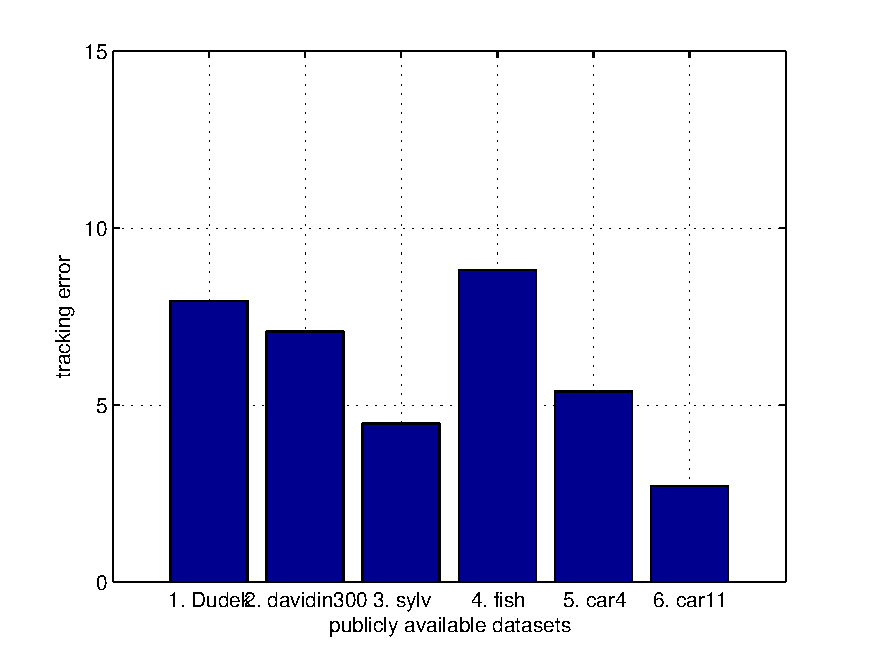
\includegraphics[width=0.45\textwidth]{temp/results_final_maxP_d.pdf}\label{fig:results_final_maxP_d}}
\caption{Tracking error for maxP based tracking for different number of codevectors per stage $M$ with fixed stages $P=8$ for 6 different publicly available datasets.}
\label{fig:results_final_maxP}
\end{figure}


%----------------------------------------------------
\clearpage
\newpage
\subsection{RofE}
%----------------------------------------------------
\begin{figure}[h!]
\centering
\begin{tabular}{|l|c|c|c|}
\hline
&\textbf{PxM=8x2}&\textbf{PxM=8x4}&\textbf{PxM=8x8}\\\hline
\textbf{Dudek}&7.11&8.43&8.19\\\hline
\textbf{davidin300}&9.02&6.21&5.74\\\hline
\textbf{sylv}&4.12&5.54&4.83\\\hline
\textbf{fish}&2.96&12.22&2.73\\\hline
\textbf{car4}&4.93&5.14&5.50\\\hline
\textbf{car11}&2.47&2.33&2.68\\\hline
\end{tabular}
\\
\subfigure[]{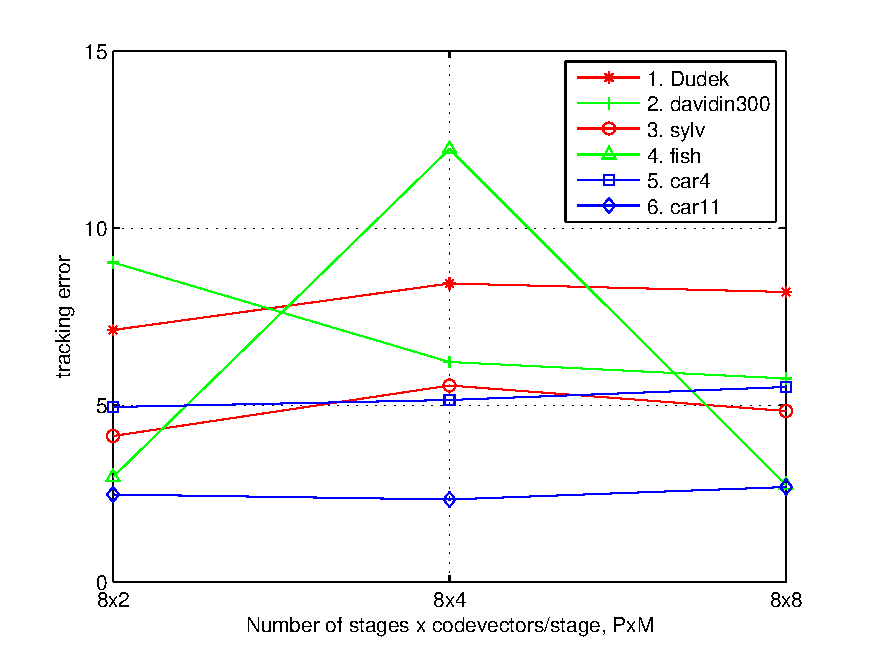
\includegraphics[width=0.45\textwidth]{temp/results_final_RofE_a.pdf}\label{fig:results_final_RofE_a}}
\subfigure[]{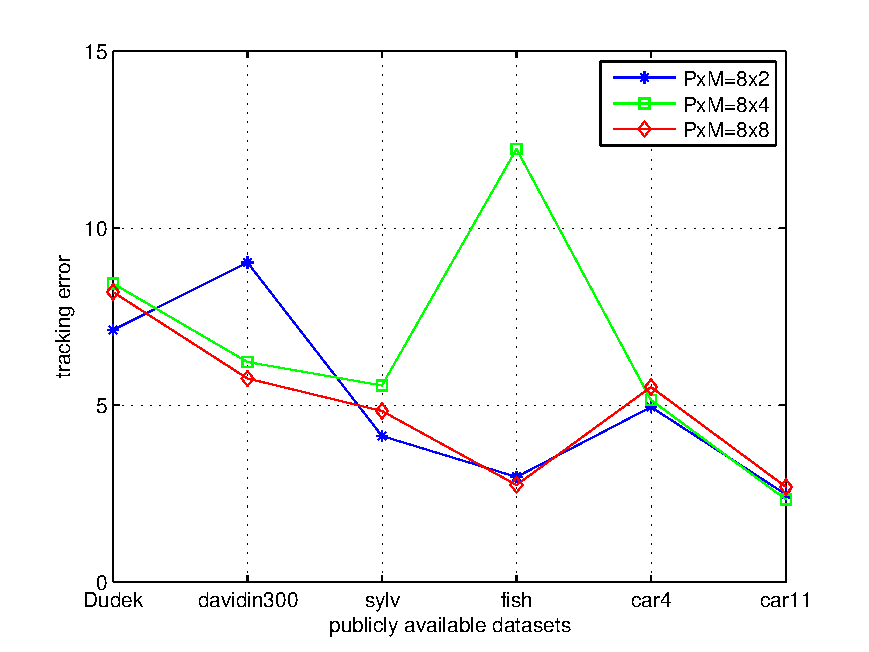
\includegraphics[width=0.45\textwidth]{temp/results_final_RofE_b.pdf}\label{fig:results_final_RofE_b}}
\subfigure[]{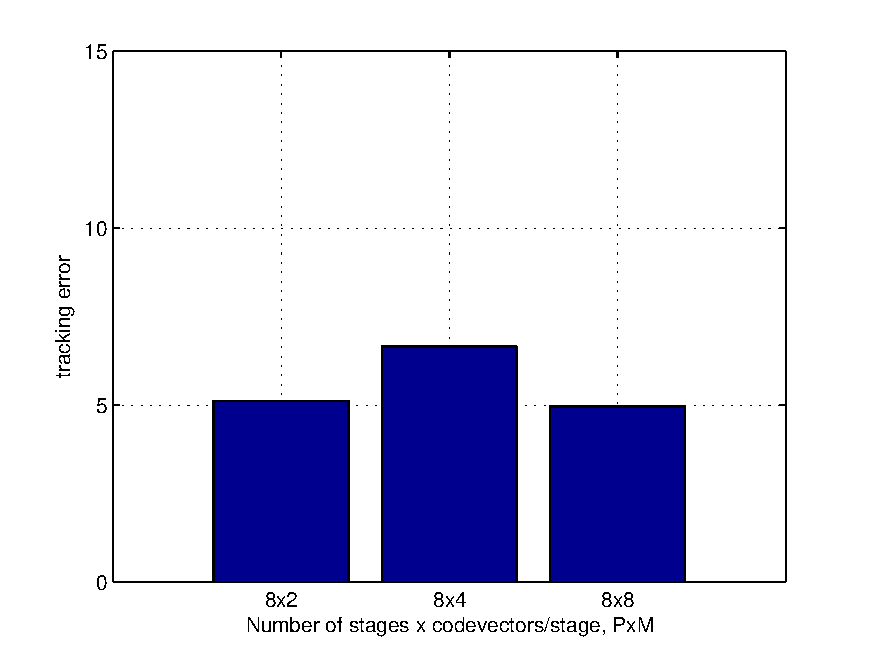
\includegraphics[width=0.45\textwidth]{temp/results_final_RofE_c.pdf}\label{fig:results_final_RofE_c}}
\subfigure[]{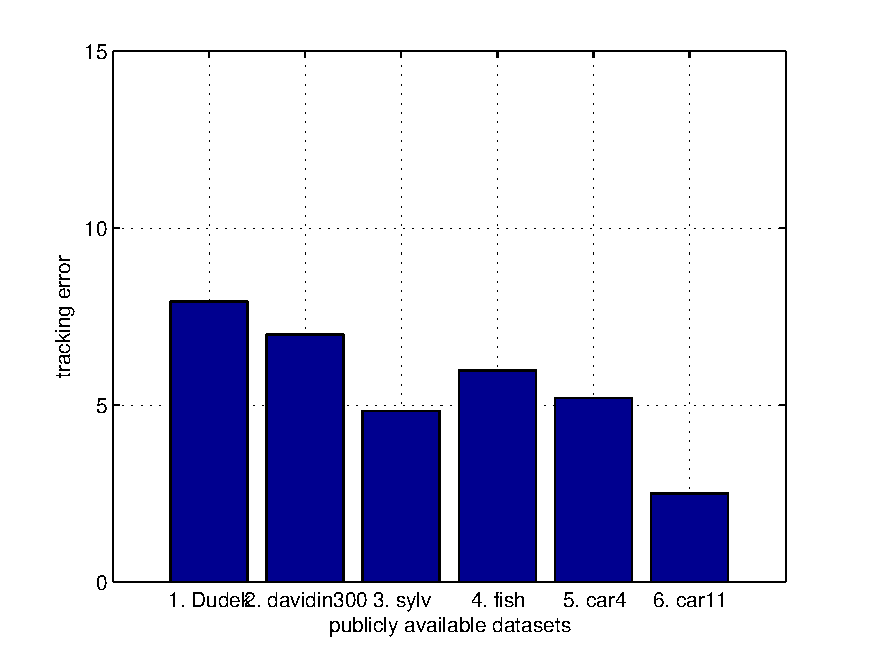
\includegraphics[width=0.45\textwidth]{temp/results_final_RofE_d.pdf}\label{fig:results_final_RofE_d}}
\caption{Tracking error for RofE based tracking for different number of codevectors per stage $M$ with fixed stages $P=8$ for 6 different publicly available datasets.}
\label{fig:results_final_RofE}
\end{figure}

%----------------------------------------------------
\clearpage
\newpage
\subsection{nulE}
%----------------------------------------------------
\begin{figure}[h!]
\centering
\begin{tabular}{|l|c|c|c|}
\hline
&\textbf{PxM=8x2}&\textbf{PxM=8x4}&\textbf{PxM=8x8}\\\hline
\textbf{1. Dudek}&9.65&8.19&7.97\\\hline
\textbf{2. davidin300}&7.17&5.35&4.63\\\hline
\textbf{3. sylv}&4.81&5.74&4.74\\\hline
\textbf{4. fish}&4.03&2.48&10.71\\\hline
\textbf{5. car4}&5.28&5.84&6.19\\\hline
\textbf{6. car11}&2.59&2.52&2.96\\\hline
\textbf{mean}&5.59&5.02&6.20\\\hline
\end{tabular}
\\
\subfigure[]{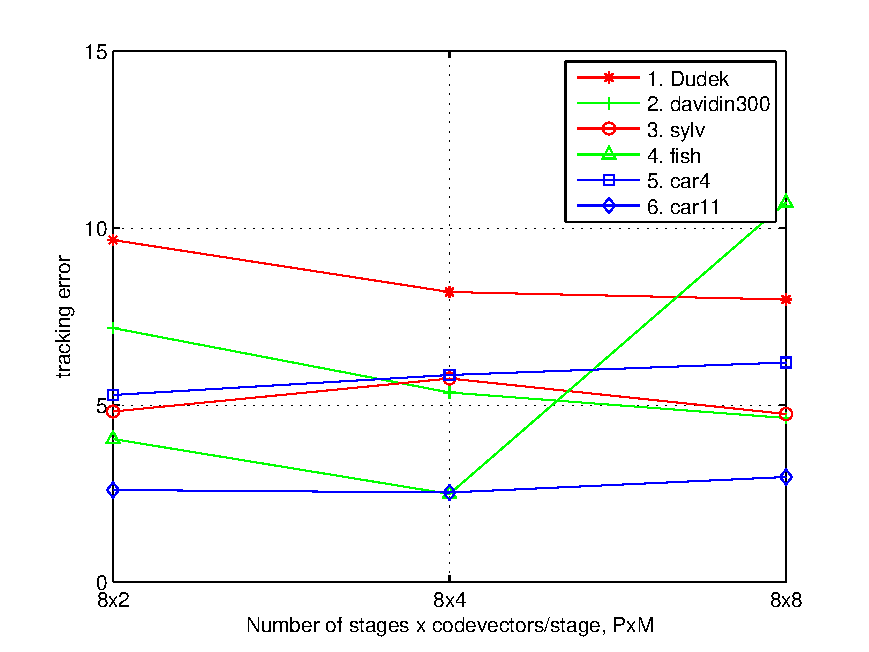
\includegraphics[width=0.45\textwidth]{temp/results_final_nulE_a.pdf}\label{fig:results_final_nulE_a}}
\subfigure[]{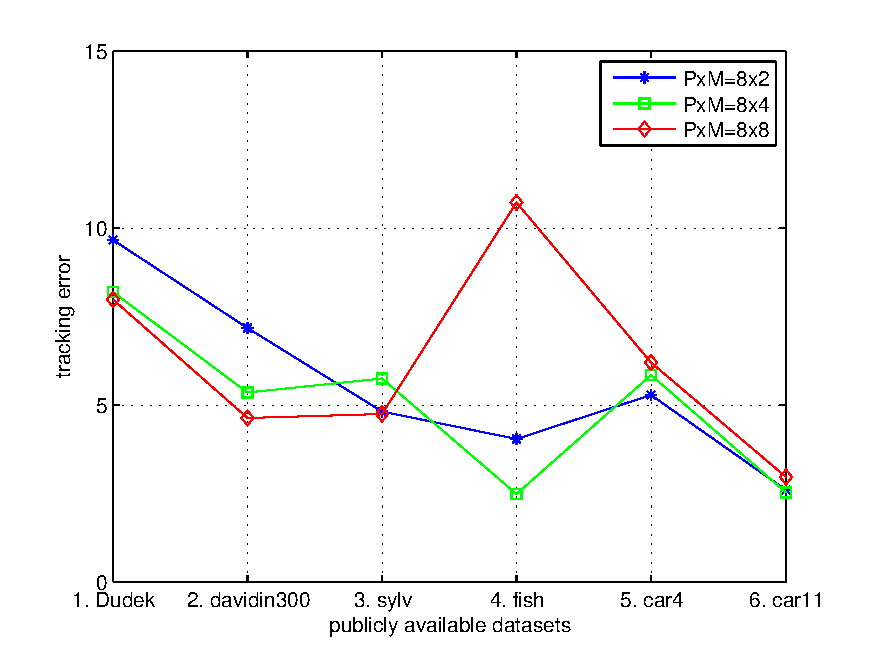
\includegraphics[width=0.45\textwidth]{temp/results_final_nulE_b.pdf}\label{fig:results_final_nulE_b}}
\subfigure[]{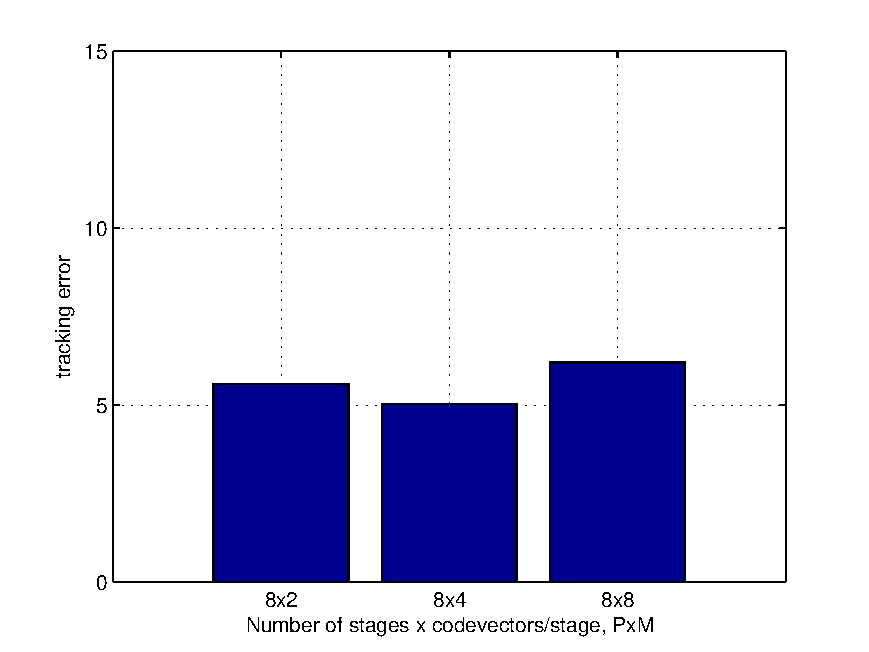
\includegraphics[width=0.45\textwidth]{temp/results_final_nulE_c.pdf}\label{fig:results_final_nulE_c}}
\subfigure[]{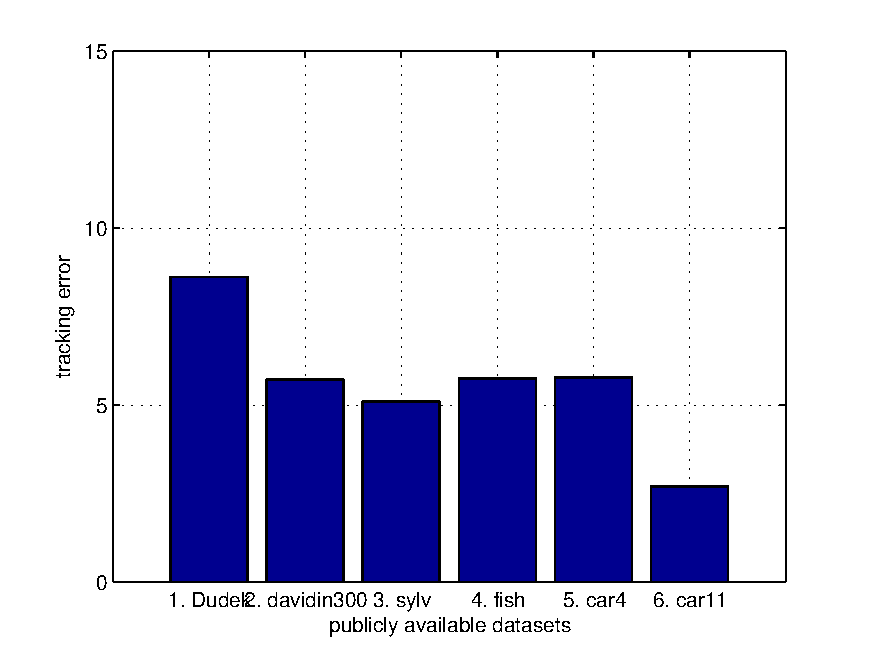
\includegraphics[width=0.45\textwidth]{temp/results_final_nulE_d.pdf}\label{fig:results_final_nulE_d}}
\caption{Tracking error for nulE based tracking for different number of codevectors per stage $M$ with fixed stages $P=8$ for 6 different publicly available datasets.}
\label{fig:results_final_nulE}
\end{figure}
%----------------------------------------------------
\clearpage
\newpage
\subsection{monR}
%----------------------------------------------------
\begin{figure}[h!]
\centering
\begin{tabular}{|l|c|c|c|}
\hline
&\textbf{PxM=8x2}&\textbf{PxM=8x4}&\textbf{PxM=8x8}\\\hline
\textbf{Dudek}&11.81&9.17&8.73\\\hline
\textbf{davidin300}&50.00&5.83&4.15\\\hline
\textbf{sylv}&4.31&4.58&5.08\\\hline
\textbf{fish}&2.89&3.62&11.94\\\hline
\textbf{car4}&5.07&5.18&4.71\\\hline
\textbf{car11}&2.47&2.72&2.55\\\hline
\end{tabular}
\\
\subfigure[]{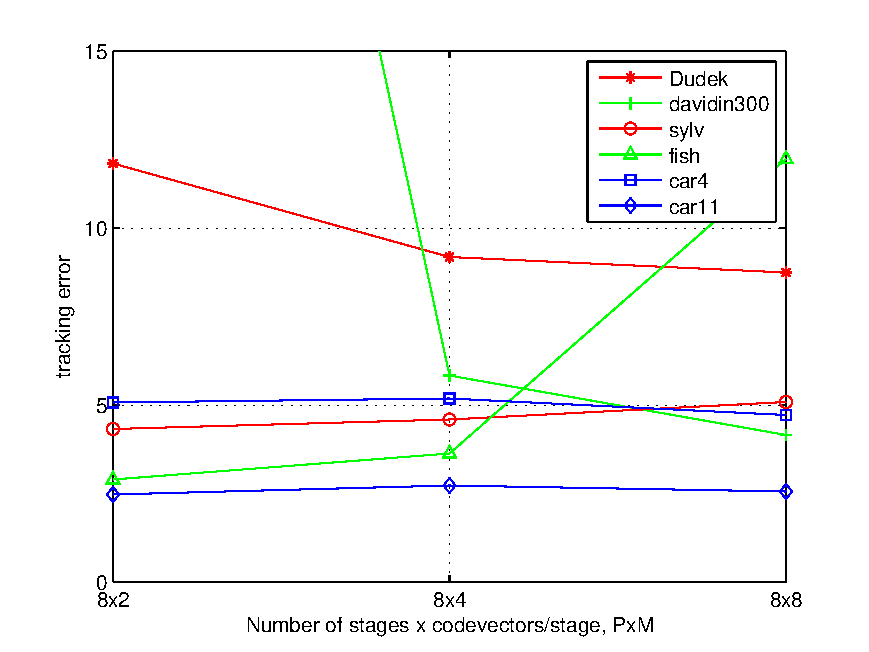
\includegraphics[width=0.45\textwidth]{temp/results_final_monR_a.pdf}\label{fig:results_final_monR_a}}
\subfigure[]{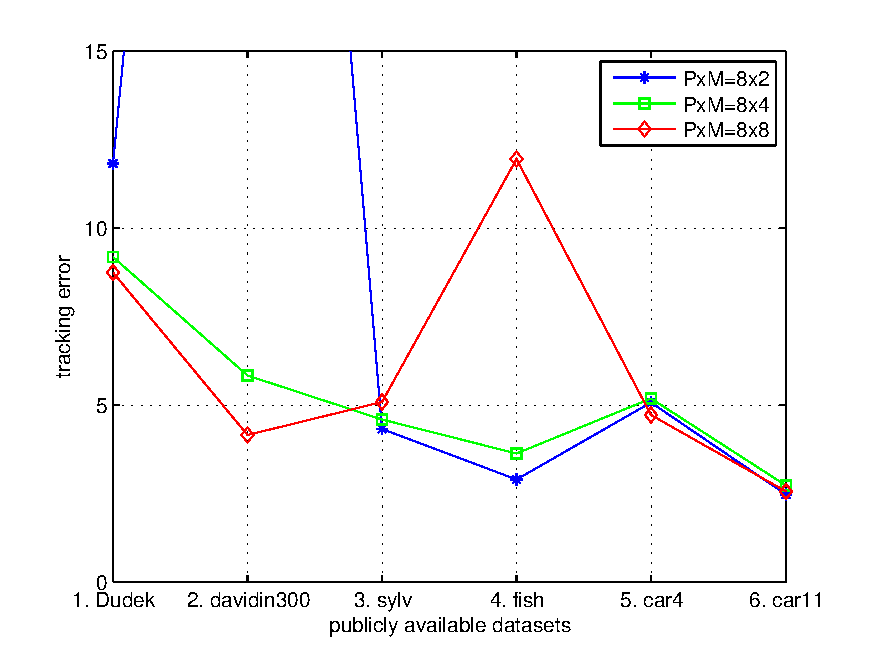
\includegraphics[width=0.45\textwidth]{temp/results_final_monR_b.pdf}\label{fig:results_final_monR_b}}
\subfigure[]{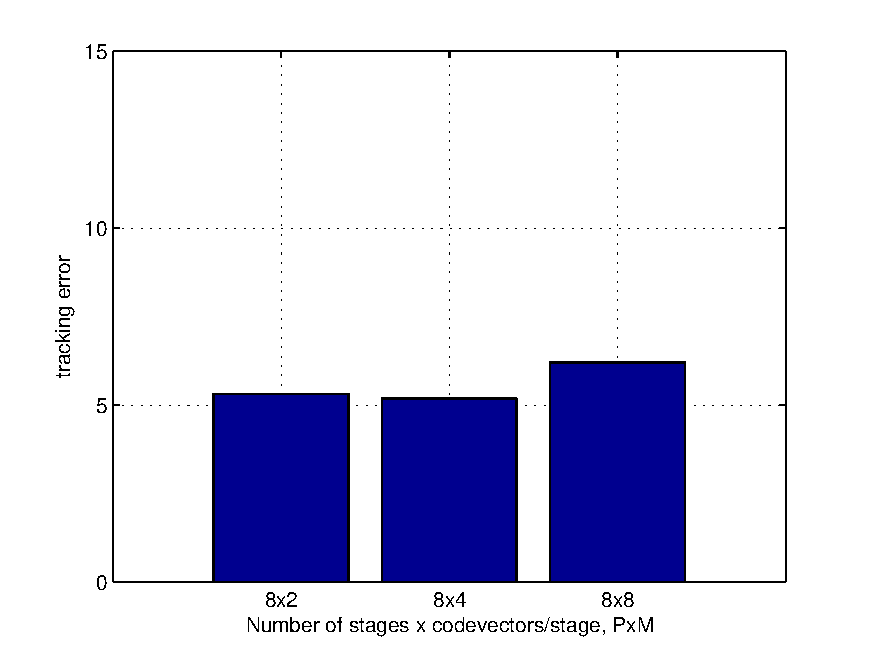
\includegraphics[width=0.45\textwidth]{temp/results_final_monR_c.pdf}\label{fig:results_final_monR_c}}
\subfigure[]{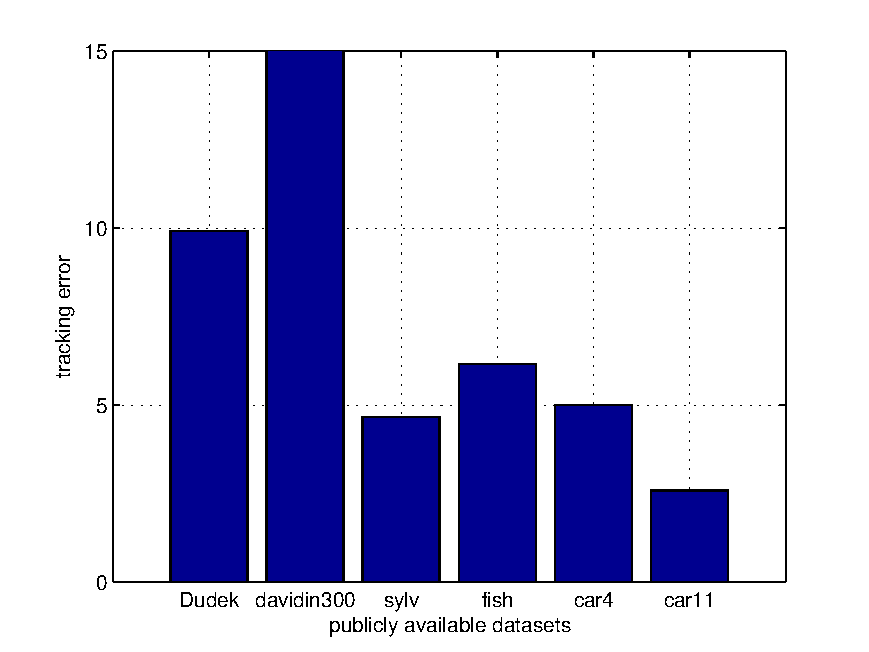
\includegraphics[width=0.45\textwidth]{temp/results_final_monR_d.pdf}\label{fig:results_final_monR_d}}
\caption{Tracking error for monR based tracking for different number of codevectors per stage $M$ with fixed stages $P=8$ for 6 different publicly available datasets. A value of 50 means that track was lost.}
\label{fig:results_final_monR}
\end{figure}

%==========================
\clearpage
\newpage
\section{Example of tracking error}
\label{App:TSVQ_Dudek_example}
%==========================
\begin{figure}[h!]
\centering
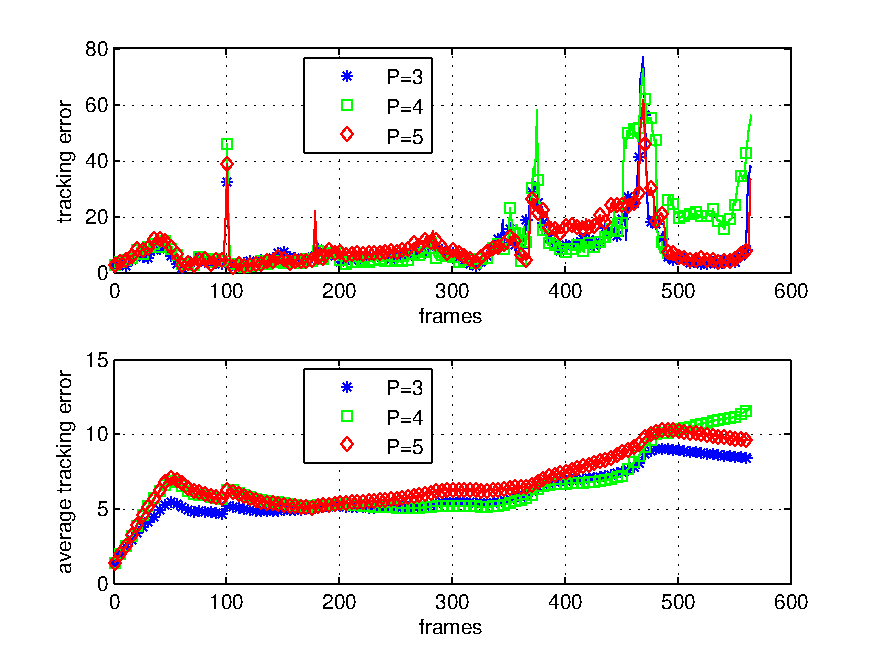
\includegraphics[width=1.0\textwidth]{temp/Dudek_TSVQ_errors.pdf}
\caption{Tracking error for TSVQ tracker, $P$=3, 4, 5, Dudek sequence.  The top figure shows instantaneous tracking error for the current frame while the bottom figure shows average tracking errors.  Notice that at frame 457, the tracker with $P=4$ makes an error which causes its average error to first exceed that of the $P$=2 tracker, and then eventually the $P$=5 tracker.}
\label{fig:results_TSVQ_Dudek_errors}
\end{figure}

\begin{figure}[h!]
\centering
\subfigure[Ground truth.]{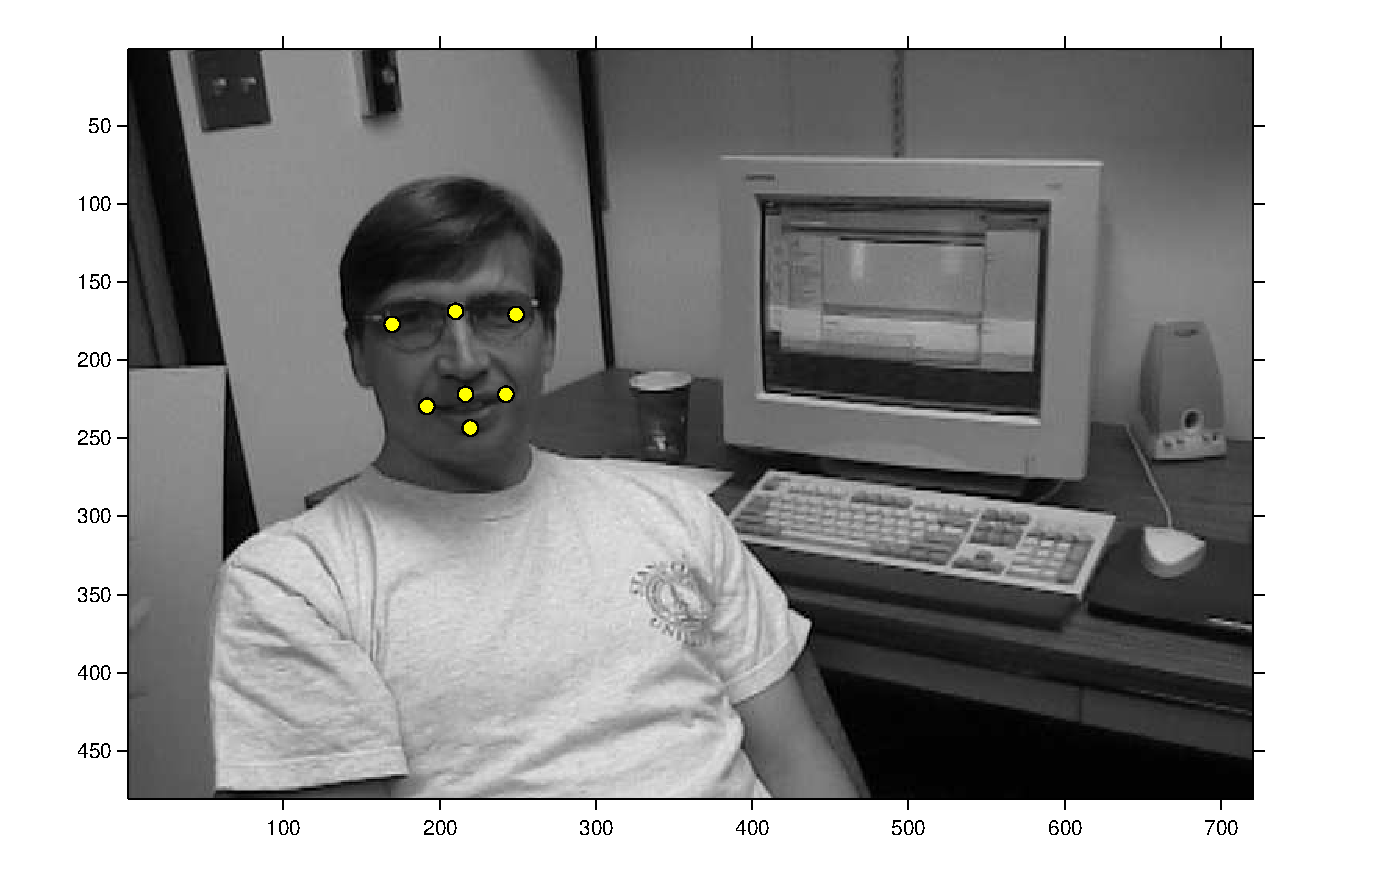
\includegraphics[width=0.3\textwidth]{temp/Dudek_GT_FN10.pdf}\label{fig:results_final_monR_b}}
\subfigure[$P$=3.]{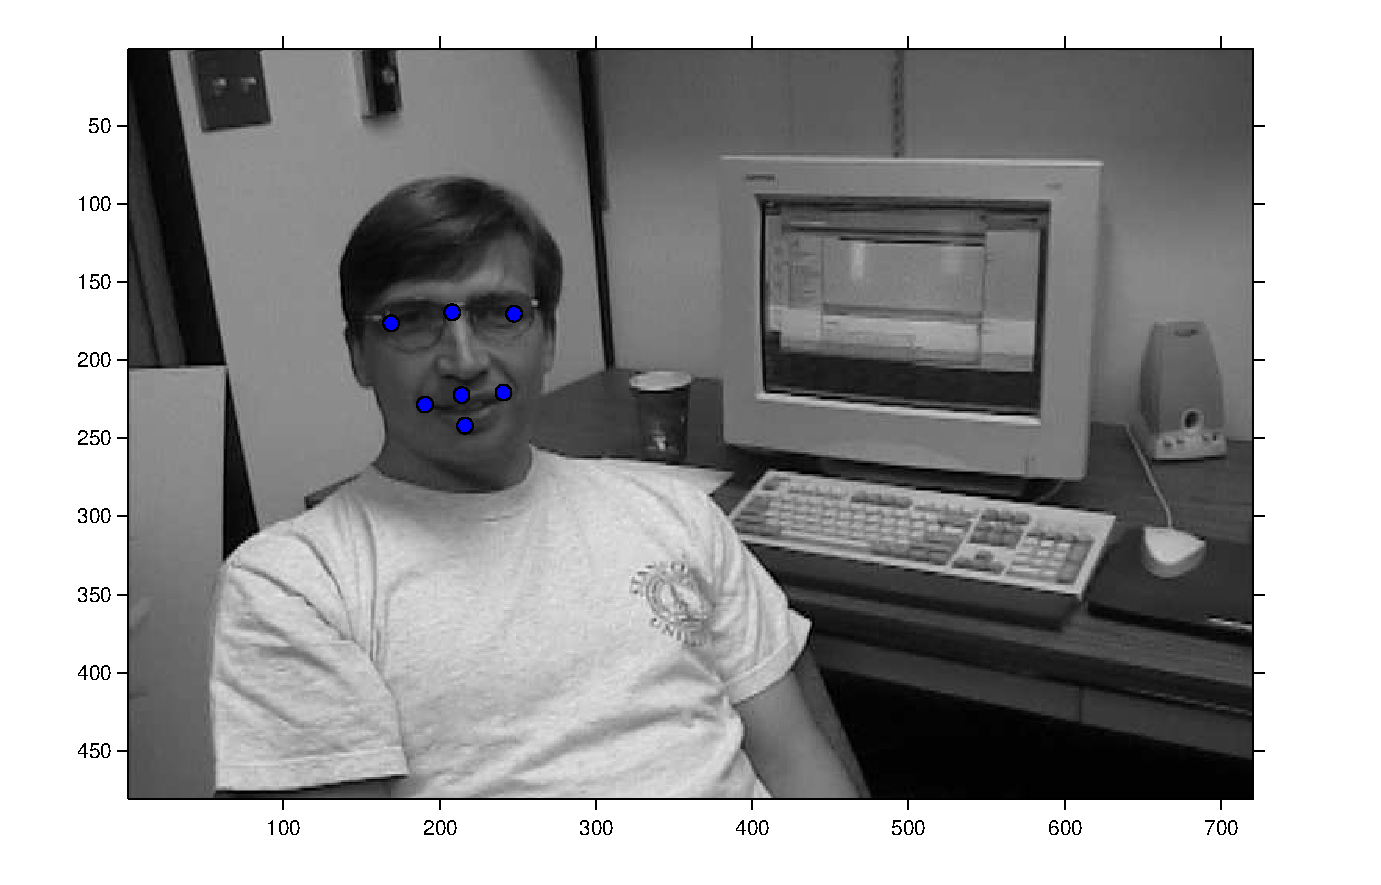
\includegraphics[width=0.3\textwidth]{temp/Dudek_TSVQ_FN10_P3.pdf}\label{fig:Dudek_TSVQ_FN10_P3}}
\subfigure[$P$=4.]{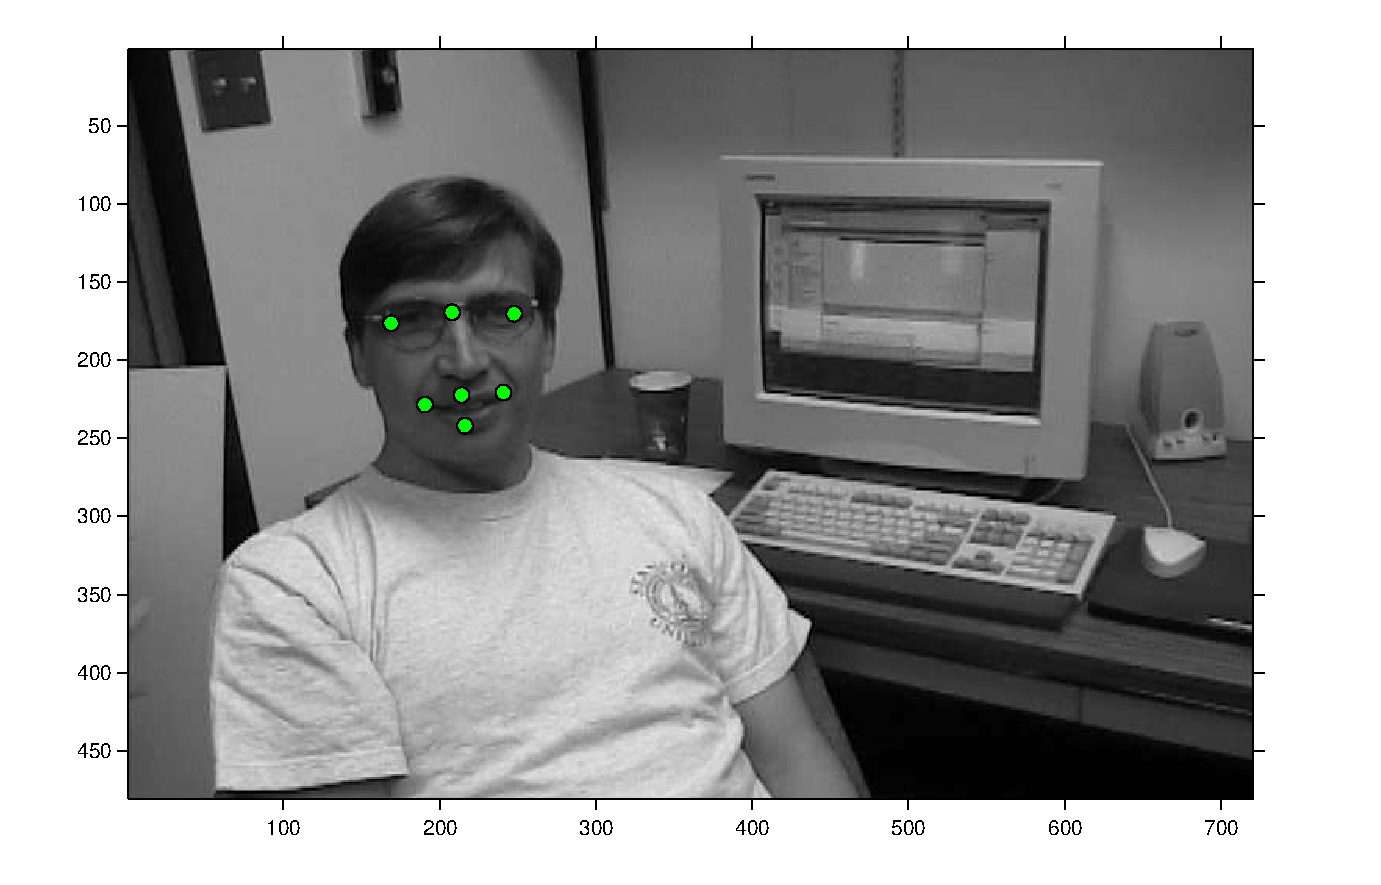
\includegraphics[width=0.3\textwidth]{temp/Dudek_TSVQ_FN10_P4.pdf}\label{fig:Dudek_TSVQ_FN10_P4}}
\subfigure[$P$=5.]{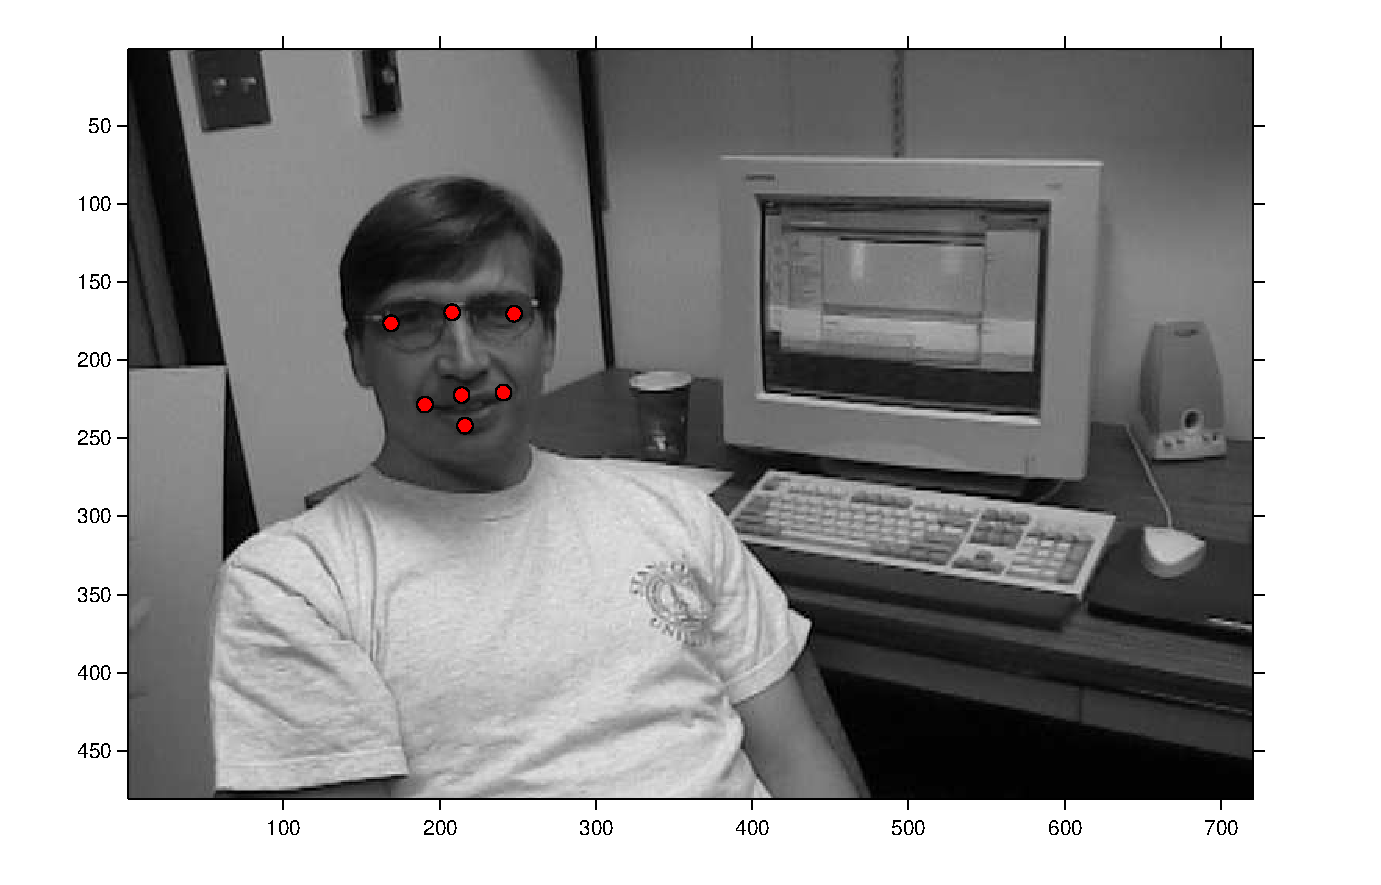
\includegraphics[width=0.3\textwidth]{temp/Dudek_TSVQ_FN10_P5.pdf}\label{fig:Dudek_TSVQ_FN10_P5}}
\caption{Low tracking error for TSVQ tracker, frame number=10.  The overlaid circles are ground truth and estimated feature points.}
\label{fig:results_TSVQ_Dudek_FN10}
\end{figure}


\begin{figure}[h!]
\centering
\subfigure[Ground truth.]{\includegraphics[width=0.3\textwidth]{temp/Dudek_GT_FN457.pdf}\label{fig:results_final_monR_b}}
\subfigure[$P$=3.]{\includegraphics[width=0.3\textwidth]{temp/Dudek_TSVQ_FN457_P3.pdf}\label{fig:Dudek_TSVQ_FN10_P3}}
\subfigure[$P$=4.]{\includegraphics[width=0.3\textwidth]{temp/Dudek_TSVQ_FN457_P4.pdf}\label{fig:Dudek_TSVQ_FN10_P4}}
\subfigure[$P$=5.]{\includegraphics[width=0.3\textwidth]{temp/Dudek_TSVQ_FN457_P5.pdf}\label{fig:Dudek_TSVQ_FN10_P5}}
\caption{High tracking error for TSVQ tracker, frame number=457.  In this frame, the person being tracked is swiftly turning his head and moving at the same time.  The tracking errors for $P$=3, 4 and 5 are 19.9, 47.3 and 25.1 respectively.  This error causes average error for $P$=4 to first exceed that of the $P$=2 tracker, and then eventually the $P$=5 tracker.  This shows that an error at a time when the target is undergoing large motion can be costly in the long term.  This is because a wrong decision can cause the wrong snippet to be included in the training set which can cause further wrong decisions.}
\label{fig:results_TSVQ_Dudek_FN457}
\end{figure}



\clearpage
\newpage
\normalsize
\bibliographystyle{ieee}
\bibliography{MyCitations}
\end{document}


